%%%%%%%%%%%%%%%%%%%%%%%%%%%%%%%%%%%%%%%%%
% Short Sectioned Assignment LaTeX Template Version 1.0 (5/5/12)
% This template has been downloaded from: http://www.LaTeXTemplates.com
% Original author:  Frits Wenneker (http://www.howtotex.com)
% License: CC BY-NC-SA 3.0 (http://creativecommons.org/licenses/by-nc-sa/3.0/)
%%%%%%%%%%%%%%%%%%%%%%%%%%%%%%%%%%%%%%%%%

% \documentclass[paper=a4, fontsize=11pt]{scrartcl} % A4 paper and 11pt font size
\documentclass[11pt, a4paper]{book}
\usepackage[T1]{fontenc} % Use 8-bit encoding that has 256 glyphs
\usepackage[utf8]{inputenc}
\usepackage{fourier} % Use the Adobe Utopia font for the document - comment this line to return to the LaTeX default
\usepackage{listings} % para insertar código con formato similar al editor
\usepackage[spanish, es-tabla]{babel} % Selecciona el español para palabras introducidas automáticamente, p.ej. "septiembre" en la fecha y especifica que se use la palabra Tabla en vez de Cuadro
\usepackage{url} % ,href} %para incluir URLs e hipervínculos dentro del texto (aunque hay que instalar href)
\usepackage{graphics,graphicx, float} %para incluir imágenes y colocarlas
\usepackage[gen]{eurosym} %para incluir el símbolo del euro
\usepackage{cite} %para incluir citas del archivo <nombre>.bib
\usepackage{enumerate}
\usepackage{hyperref}
\usepackage{graphicx}
\usepackage{tabularx}
\usepackage{booktabs}
\usepackage[margin=3cm]{geometry}
\usepackage{array}
\usepackage{graphicx}
\usepackage{rotating}
\usepackage{amsmath}
\usepackage{amssymb}
\usepackage{mathrsfs}
\usepackage{listings}
\usepackage{xcolor}  

\usepackage{todonotes}
\usepackage{ulem}
\newcommand{\Beni}[2][]{\todo[inline, color=purple!30, caption={ToDo - Benigno}, #1]{\begin{minipage}{\textwidth-4pt} #2\\ {\bf  -- Benigno} \end{minipage}}}
\newcommand{\Juanlu}[2][]{\todo[inline, color=red!20, caption={ToDo - Juanlu}, #1]{\begin{minipage}{\textwidth-4pt} #2 {\bf -- Juanlu}\end{minipage}}}

\lstdefinestyle{mystyle}{
    backgroundcolor=\color{gray!10},
    commentstyle=\color{green!50!black},
    keywordstyle=\color{blue},
    numberstyle=\tiny\color{gray},
    stringstyle=\color{orange},
    basicstyle=\ttfamily\footnotesize,
    breaklines=true,
    numbers=left,
    numbersep=5pt,
    frame=single,
    rulecolor=\color{black},
    tabsize=2,
    showstringspaces=false
}
\lstset{style=mystyle}


\usepackage[table,xcdraw]{xcolor}
\hypersetup{
	colorlinks=true,	% false: boxed links; true: colored links
	linkcolor=black,	% color of internal links
	urlcolor=cyan		% color of external links
}
\renewcommand{\familydefault}{\sfdefault}
\usepackage{fancyhdr} % Custom headers and footers
\pagestyle{fancyplain} % Makes all pages in the document conform to the custom headers and footers
\fancyhead[L]{} % Empty left header
\fancyhead[C]{} % Empty center header
\fancyhead[R]{\nouppercase{\leftmark}} % Sección actual a la derecha
\fancyfoot[L]{} % Empty left footer
\fancyfoot[C]{} % Empty center footer
\fancyfoot[R]{\thepage} % Page numbering for right footer
%\renewcommand{\headrulewidth}{0pt} % Remove header underlines
\renewcommand{\footrulewidth}{0pt} % Remove footer underlines
\setlength{\headheight}{13.6pt} % Customize the height of the header

\usepackage{titlesec, blindtext, color}
\definecolor{gray75}{gray}{0.75}
\newcommand{\hsp}{\hspace{20pt}}
\titleformat{\chapter}[hang]{\Huge\bfseries}{\thechapter\hsp\textcolor{gray75}{|}\hsp}{0pt}{\Huge\bfseries}
\setcounter{secnumdepth}{4}
\usepackage[Lenny]{fncychap}


\begin{document}

	% Plantilla portada UGR
	\begin{titlepage}
 
 
\newlength{\centeroffset}
\setlength{\centeroffset}{-0.5\oddsidemargin}
\addtolength{\centeroffset}{0.5\evensidemargin}
\thispagestyle{empty}

\noindent\hspace*{\centeroffset}\begin{minipage}{\textwidth}

\centering

\includegraphics[width=0.9\textwidth]{imagenes/logo_ugr.jpg}\\[1.4cm]

\textsc{ \Large TRABAJO FIN DE GRADO\\[0.2cm]}
\textsc{ GRADO EN INGENIERIA INFORMATICA}\\[1cm]

{\huge\bfseries Análisis de desempeño y predicción de resultados en fútbol mediante mapas de calor \\}
\noindent\rule[-1ex]{\textwidth}{3pt}\\[3.5ex]
\end{minipage}

\vspace{2.5cm}
\noindent\hspace*{\centeroffset}
\begin{minipage}{\textwidth}
\centering

\textbf{Autor}\\ {Benigno Joaquín Parra Campos}\\[2.5ex]
\textbf{Director}\\ {Javier Medina Quero, Juan Luis Jiménez Laredo}\\[2cm]

\includegraphics[width=0.3\textwidth]{imagenes/etsiit_logo.png}\\[0.1cm]
\textsc{Escuela Técnica Superior de Ingenierías Informática y de Telecomunicación}\\
\textsc{---}\\
Granada, Junio de 2025
\end{minipage}
%\addtolength{\textwidth}{\centeroffset}
%\vspace{\stretch{2}}
\end{titlepage}



	% Plantilla prefacio UGR
	\thispagestyle{empty}

\begin{center}
{\large\bfseries Título \\ Subtítulo }\\
\end{center}
\begin{center}
Nombre Del Estudiante\\
\end{center}

%\vspace{0.7cm}

\vspace{0.5cm}
\noindent\textbf{Palabras clave}: \textit{software libre}
\vspace{0.7cm}

\noindent\textbf{Resumen}\\
	

\cleardoublepage

\begin{center}
	{\large\bfseries Same, but in English}\\
\end{center}
\begin{center}
	Student's name\\
\end{center}
\vspace{0.5cm}
\noindent\textbf{Keywords}: \textit{open source}, \textit{floss}
\vspace{0.7cm}

\noindent\textbf{Abstract}\\


\cleardoublepage

\thispagestyle{empty}

\noindent\rule[-1ex]{\textwidth}{2pt}\\[4.5ex]

D. \textbf{Tutora/e(s)}, Profesor(a) del ...

\vspace{0.5cm}

\textbf{Informo:}

\vspace{0.5cm}

Que el presente trabajo, titulado \textit{\textbf{Chief}},
ha sido realizado bajo mi supervisión por \textbf{Estudiante}, y autorizo la defensa de dicho trabajo ante el tribunal
que corresponda.

\vspace{0.5cm}

Y para que conste, expiden y firman el presente informe en Granada a Junio de 2018.

\vspace{1cm}

\textbf{El/la director(a)/es: }

\vspace{5cm}

\noindent \textbf{(nombre completo tutor/a/es)}

\chapter*{Agradecimientos}






	% Índice de contenidos
	\newpage
	\tableofcontents

	% Índice de imágenes y tablas
	\newpage
	\listoffigures

	% Si hay suficientes se incluirá dicho índice
	\listoftables 
	\newpage

	% Introducción 
	\chapter{Introducción}

Este proyecto es software libre, y está liberado con la licencia \cite{gplv3}.

	% Estado del arte
	% 	1. Crítica al estado del arte
	% 	2. Propuesta
	\chapter{Estado del arte}

El fútbol es un deporte altamente impredecible, en el que incluso los detalles más pequeños pueden tener un impacto significativo en el resultado de un partido. Dada la complejidad del juego y la cantidad de variables implicadas, resulta esencial identificar qué áreas han sido objeto de estudio mediante técnicas de aprendizaje automático y cuáles presentan aún oportunidades para futuras investigaciones. Al finalizar este trabajo, se contará con una visión general y estructurada sobre los aspectos del fútbol que han sido previamente explorados, así como aquellos que permanecen relativamente inexplorados. Para la recopilación de información, se han utilizado filtros de búsqueda aplicados a términos relacionados con 'football' o 'soccer', combinados con 'machine learning' o 'deep learning'.

Como criterios de inclusión y exclusión se han usado los siguientes:
\begin{itemize}
    \item Individuos: Los participantes analizados deben ser exclusivamente jugadores de fútbol. No obstante, también se aceptan estudios que incluyan múltiples disciplinas deportivas, siempre que se puedan extraer y utilizar únicamente los datos correspondientes al fútbol.
    \item Técnica: Los datos han tenido que ser procesados mediante \textit{machine learning} o \textit{deep learning} y no mediante otras técnicas.
    \item Predicción: La predicción debe centrarse en el rendimiento individual o colectivo de los jugadores, excluyendo cualquier otro ámbito ajeno al mundo del fútbol, como aspectos económicos o políticos.
    \item Idioma: los textos son escritos originalmente en inglés y no en otro idioma, o hechos basados en otros artículos originales.
\end{itemize}

Como puede observarse, los criterios de inclusión y exclusión han sido definidos con el objetivo de centrarse exclusivamente en el ámbito del fútbol y en los datos relativos a los futbolistas, al mismo tiempo que se asegura la selección de estudios de calidad.

\section{Revisión de la literatura}

En el ámbito del fútbol, la investigación basada en datos se ha centrado principalmente en tres grandes áreas: la predicción de lesiones en los futbolistas, la estimación de los resultados de los partidos y el pronóstico del desarrollo de la carrera deportiva de jugadores individuales. Estas categorías agrupan la mayoría de los estudios recientes orientados al análisis y la predicción dentro de este deporte.

Cada una de estas categorías abarca a su vez diferentes enfoques y subdivisiones específicas, las cuales se irán desarrollando a lo largo de esta sección con el objetivo de ofrecer una visión general del estado actual de la investigación en este ámbito.

El primer tema a tratar es el de las lesiones en futbolistas. Diversos estudios han intentado predecir su aparición, identificando los factores más comunes con el objetivo de prevenirlas. Una de las lesiones más frecuentes es la distensión de isquiotibiales. En el estudio realizado por Ayala et al. \cite{first-injury}, se analizaron 96 jugadores profesionales pertenecientes a 18 equipos distintos, teniendo en cuenta variables como la pierna dominante, el estado psicológico del jugador y otros atributos físicos medibles, como la fuerza o la flexibilidad. Utilizando un algoritmo de \textit{machine learning} AD Tree, llegaron a la conclusión de que, con más de un 78\% de probabilidad, sí había factores que eran predominantes en las 18 lesiones que detectaron, entre ellos la calidad del sueño, el historial de lesiones de isquiotibial o el ángulo de su rodilla al golpear el balón.

En este otro estudio de López-Valenciano \textit{et al.} \cite{second-injury}, se analizaron a 98 jugadores de 4 equipos diferentes y se tuvieron en cuenta factores idénticos al anterior. Su objetivo era minimizar una lesión de cualquier músculo del cuerpo, y para ello utilizaron 4 árboles de decisión que fueron C4.5, SimpleCart, ADTree y RandomTree. Los resultados obtenidos indican que, con un 66\% de probabilidad, podrían ayudar a los entrenadores en la reducción de las lesiones de sus jugadores mediante la modificación de los entrenamientos al detectar posibles riesgos en algunos ejercicios determinados. En este estudio de Rommers \textit{et al.} \cite{third-injury}, se analizaron a 734 niños de entre 10 y 15 años durante una temporada entera. Su objetivo era predecir las lesiones por sobrecarga en los músculos, por lo que se tomaron medidas como la altura, peso, velocidad, resistencia, etc. Utilizaron un algoritmo XGBoost y con una precisión entre el 75\% y 85\% pudieron predecir qué jugadores eran los que tenían más riesgo de lesión.

Como se puede apreciar, en el ámbito de las lesiones se han hecho varios estudios, y la mayoría de ellos son exitosos, lo que nos lleva a pensar que es un campo ya explorado, pero a su vez nos indica que hay campos dentro del fútbol que sí se pueden predecir con precisión.

Vamos ahora a analizar aquellos estudios relacionados con la predicción de partidos o de eventos que ocurran dentro de partidos. En este primer estudio de Dick y Brefeld \cite{first-outcome}, se analizaron 5 partidos de ligas de fútbol profesional con gran variedad de ataques, los cuales 380 fueron exitosos y 715 no lo fueron. Su objetivo era predecir qué situaciones del juego son las más favorables para tener un ataque exitoso. Un ataque exitoso se entiende como aquel en el que el balón está a menos de 25 metros de la portería rival. Para ello, utilizan algunos atributos como la posesión del equipo, las posiciones de cada uno de los jugadores con coordenadas X e Y y el tiempo de juego efectivo, utilizando el algoritmo de optimización de Adam (Adaptive Moment Estimation). Finalmente, llegaron a la conclusión de que, aparte de saber qué ataques podrían ser exitosos, también podría utilizarse para evaluar la posición de los jugadores y la velocidad de los ataques. En este otro estudio mucho más grande de Goes \textit{et al.} \cite{second-outcome}, se analizaron a 26 equipos profesionales durante 4 temporadas y contabilizaron 1.237 ataques exitosos y 11.187 que no lo fueron. Mediante un sistema de video semiautomático, analizaron el centro geométrico entre las distintas líneas del equipo, sobre todo del portero con la defensa y la defensa con los centrocampistas. Se utilizó un algoritmo de k-medias, y se llegó a la conclusión de que, aplicando el centro geométrico a las líneas del equipo en vez de al equipo entero en su totalidad, es más preciso a la hora de predecir ataques exitosos, así como que los ataques exitosos dependen de que los defensores creen espacio para los atacantes y de que estén sincronizados con los centrocampistas.

En el estudio presentado por AlMulla \textit{et al.} en \cite{third-outcome}, se analizaron partidos de la liga catarí disputados entre 2011 y 2022, utilizando datos históricos de los jugadores que participaron en dichos encuentros. Mediante el uso de redes neuronales GRU (Gated Recurrent Units), se logró predecir el equipo ganador con una precisión del 80\%. Además, el análisis se extendió al desempeño de los jugadores en distintas fases del partido, concluyéndose que los defensores desempeñan un papel determinante en el resultado final. Asimismo, se identificó que los intervalos temporales comprendidos entre los minutos 15 y 30 de cada mitad son los más significativos en términos de impacto en el rendimiento general del equipo.

Como se puede observar, estos estudios se centran en el análisis de ataques exitosos y en la predicción del equipo ganador. No obstante, se basan únicamente en estadísticas individuales de los jugadores, sin considerar su relación con las zonas del campo en las que han estado presentes.

Ahora vamos a pasar a analizar 2 estudios sobre los pases de los jugadores. En el primero de ellos, de Szczepańsk y McHale \cite{first-passes}, analizan 760 partidos durante 2 temporadas en la primera división inglesa, teniendo en cuenta cuál es la calidad del jugador que da el pase y su situación antes de darlo. Su objetivo es predecir la dificultad del pase y la probabilidad de que este sea exitoso, y para ello utilizan un algoritmo de naive bayes. El estudio es exitoso y consigue detectar quiénes serían los mejores pasadores. En este otro estudio más preciso de Chawla \textit{et al.} \cite{second-passes}, se analizó al equipo de fútbol 'Arsenal' durante 4 partidos de la primera división inglesa para intentar predecir sus pases. Utilizando un sistema de cámaras y de observadores humanos, contabilizaron 2.932 pases durante el análisis. Para la predicción se tuvieron en cuenta factores como la trayectoria que sigue el jugador en el campo, los toques al balón, pases, tiros y mapas donde dominaba más cada jugador. Para el algoritmo utilizaron un RUSBoost classifier y un multinomial logistic regression y con más de un 90\% de precisión consideraron que sí podían predecir cómo de bueno iba a ser un pase que se iba a dar.

En estos estudios se logró predecir con éxito la calidad y efectividad de los pases, considerando atributos del jugador como su posición en el campo. Sin embargo, dicha técnica no se extendió al ámbito de la predicción del resultado de los partidos.

Después se realizaron otros estudios como el de Link y Hoernig \cite{first-other}, donde se analizaron 60 partidos de la liga alemana, con un total de casi 70.000 acciones captadas mediante un sistema de cámaras semiautomático. Tuvieron en cuenta la posición de los jugadores, posesión del equipo, posesión individual y acciones individuales y colectivas con el balón. Querían determinar cuánto tiempo pasa el balón en la esfera de influencia de un jugador, basándose en la distancia entre los jugadores y el balón, junto con su dirección de movimiento, velocidad y aceleración. Se hace mediante la configuración espacio-temporal del jugador que controla el balón utilizando redes bayesianas. El estudio llega a la conclusión de que podemos saber durante cuánto tiempo ha estado el balón en la esfera de influencia de un futbolista y conocer su influencia en el juego.

En este otro estudio de Montoliu \textit{et al.} \cite{second-other}, se analizaron cuatro equipos de la primera división española durante cuatro temporadas y se tuvieron en cuenta durante los ataques del equipo la posesión del balón, los regates, desmarques, así como los libres directos e indirectos. Su objetivo era predecir cuál sería el patrón de ataque del equipo tanto en jugadas de posesión como a balón parado. Utilizaron un algoritmo de random forest y k-vecinos más cercanos y, entre una precisión entre 67\% y 93\%, podían predecir cuál sería el patrón de ataque del equipo. Este otro estudio de Knauf \textit{et al.} \cite{third-other}, también analiza los patrones de un equipo; para ello, analizó 10 partidos de primera y segunda división alemana durante una temporada, y tuvo en cuenta la trayectoria del jugador en el campo y las oportunidades de gol en el último cuarto del campo. Utilizaron un algoritmo k-medoids y finalmente pudieron predecir si los ataques iban a ser lentos o rápidos, así como la cantidad de pases por ataque.

Predecir patrones de ataque parece ser exitoso utilizando \textit{machine learning}, por lo que nos indica que esta es ya otra área explorada del fútbol.

Por otro lado, existen diversos estudios que analizan la posible trayectoria de un futbolista a lo largo de su carrera profesional. Uno de ellos es el trabajo presentado por Barron \textit{et al.} en \cite{first-career}, en el que se estudia una muestra de 966 jugadores: 209 no profesionales, 637 pertenecientes a la segunda división inglesa y 120 a la primera división inglesa. En este estudio se tienen en cuenta variables como el número de pases, su precisión y consistencia, así como entradas, duelos ganados y tiros. El objetivo principal es predecir el nivel futuro del jugador y la división en la que podría competir en la siguiente temporada, utilizando para ello una red neuronal artificial (ANN). Los resultados muestran una precisión de entre el 69\% y el 77\% en la predicción de la división futura y la trayectoria profesional del jugador a medio plazo.

En otro estudio relevante de Ćwiklinski \textit{et al.} \cite{second-career}, se analizaron 4.700 jugadores pertenecientes a 156 equipos de las ocho principales ligas europeas. Este trabajo considera un total de 29 atributos técnicos, variables psicológicas y datos de rendimiento en partidos anteriores. El objetivo es predecir si la transferencia de un jugador entre dos clubes será exitosa, entendiéndose como tal una mejora en el rendimiento del jugador respecto a su temporada anterior. Para ello, se emplean algoritmos como Random Forest, Naive Bayes y AdaBoost. Aunque los resultados permiten estimar el posible éxito de una transferencia, los autores destacan que estos deben interpretarse más como recomendaciones que como predicciones absolutas.

Otra dimensión interesante de predicción en el fútbol es la elaboración de alineaciones. Aunque existen pocos estudios centrados en este aspecto, uno de ellos, hecho por García-Aliaga \textit{et al.} \cite{starting-up}, analiza más de 50.000 partidos y 30.000 jugadores a lo largo de siete temporadas en 18 ligas nacionales distintas. El objetivo del estudio es determinar cuál sería la posición óptima para cada jugador, teniendo en cuenta sus características individuales, con el fin de maximizar su rendimiento. Para ello, se emplea el algoritmo RIPPER (Repeated Incremental Pruning to Produce Error Reduction), logrando una precisión superior al 73\% en la predicción de la posición más adecuada para cada jugador. Estos resultados pueden resultar especialmente útiles a la hora de diseñar alineaciones más eficaces.

Como se ha podido observar, existen numerosos ámbitos en los que el aprendizaje automático se aplica con éxito en el contexto del fútbol. No obstante, aunque algunos estudios mencionan la posibilidad de generar mapas de calor que reflejen la influencia espacial de cada jugador, ninguno de ellos los utiliza directamente como herramienta para la predicción. Del mismo modo, aunque hay investigaciones que intentan predecir el resultado de un partido a partir de ciertos atributos, no se establece ninguna relación con los mapas de calor que muestran las zonas del campo donde ha intervenido cada jugador.

\section{Contribuciones de este trabajo}
El análisis del estado del arte ha permitido identificar múltiples enfoques aplicados al ámbito del fútbol, como el uso de datos estadísticos, modelos de \textit{machine learning} para la predicción de resultados y representaciones visuales como los mapas de calor. No obstante, se ha detectado una carencia significativa de estudios que combinen de forma sistemática las características individuales de los jugadores con su posicionamiento e influencia espacial durante el partido.

En este contexto, las principales contribuciones de este Trabajo de Fin de Grado son las siguientes:

\begin{itemize}
    \item Integración del rendimiento individual y espacial: Se propone un modelo que relaciona los atributos individuales de los jugadores con su distribución en el terreno de juego, utilizando mapas de calor como fuente principal de información contextual.
    \item Aplicación de técnicas de \textit{machine learning} a datos espaciales específicos: Frente a estudios previos centrados en estadísticas generales o resultados de equipo, este trabajo aplica algoritmos de aprendizaje automático sobre datos derivados directamente de la actividad espacial de los futbolistas, con el objetivo de identificar patrones relevantes en relación con el rendimiento y el resultado del partido.
    \item Exploración de un área poco abordada: Al centrarse en el análisis de mapas de calor como herramienta predictiva, este trabajo abre una línea de investigación emergente que ha sido poco explorada en la literatura existente.
    \item Base para desarrollos futuros: La metodología desarrollada, junto con los resultados obtenidos, sienta las bases para futuras ampliaciones, como el aumento del volumen de datos, la incorporación de nuevas variables contextuales o la aplicación a competiciones y niveles distintos.
\end{itemize}

Estas contribuciones permiten situar este trabajo dentro del campo de la analítica deportiva, proporcionando un enfoque novedoso que combina el análisis espacial y estadístico con técnicas avanzadas de predicción.

	
	\chapter{Planificación}

\section{Metodología utilizada}
Para la organización y desarrollo de este TFG se ha optado por seguir una metodología ágil, concretamente el marco de trabajo SCRUM. Esta elección permite estructurar el proyecto en ciclos iterativos e incrementales, favoreciendo la adaptabilidad, el control del progreso y la mejora continua.

El proyecto se ha dividido en tres iteraciones principales, cada una con una duración determinada y unos objetivos específicos. 

Esta planificación permite mantener una visión clara del desarrollo del trabajo, asegurando que se cumplen los plazos establecidos y que se cubren progresivamente todos los aspectos necesarios del proyecto, desde la recolección y análisis de datos hasta el diseño y validación del modelo propuesto.

En total, se han definido 17 historias de usuario para el proyecto. Cada una de ellas cuenta con una estimación del esfuerzo necesario, basada en la escala de Fibonacci. Además, se les ha asignado un nivel de prioridad, que puede ser: muy alta, alta, media o baja. Las historias están ordenadas según el cronograma previsto de desarrollo, aunque este orden puede modificarse en función de las necesidades del proyecto.

\begin{table}[h]
    \centering
    \begin{tabular}{|>{\centering\arraybackslash}p{1.5cm}|>{\centering\arraybackslash}p{6cm}|>{\centering\arraybackslash}p{2cm}|>{\centering\arraybackslash}p{1.8cm}|}
        \hline
        \textbf{ID} & \textbf{Historia de Usuario} & \textbf{Prioridad} & \textbf{Estimación} \\ \hline
        HU.01 & Reunión inicial con tutores & Muy alta & 2 \\ \hline
        HU.02 & Revisión de la literatura & Alta & 13\\ \hline
        HU.03 & Redacción del estado del arte& Alta & 8\\ \hline
        HU.04 & Definición de las estadísticas a almacenar & Alta & 3 \\ \hline
        HU.05 & Diseño de la base de datos & Alta & 5\\ \hline
        HU.06 & Implementación de programa para recolectar datos & Alta & 8\\ \hline
        HU.07 & Diseño de algoritmo para definir ganador& Alta & 8 \\ \hline
        HU.08 & Implementación algoritmo para definir ganador por pesos& Alta & 5\\ \hline
        HU.09 & Implemetación programa básico sin pesos & Media & 2 \\ \hline
        HU.10 & Análisis de las variables del agoritmo genético & Media & 5 \\ \hline
        HU.11 & Implementación del algoritmo genético por pesos & Alta & 5 \\ \hline
        HU.12 & Implementación del algoritmo genético por pesos y delta & Alta & 5 \\ \hline
        HU.13 & Análisis de los datos recogidas por los algoritmos& Alta & 8\\ \hline
        HU.14 & Diseño algoritmo para obtención de datos individuales del partido & Baja & 3 \\ \hline
        HU.15 & Implemetación del algoritmo para obtención de datos individuales del partido& Baja & 5 \\ \hline
        HU.16 & Análisis de los datos de cada jugador individual& Baja & 5 \\ \hline
        HU.17 & Redacción de la memoria & Alta & 8 \\ \hline
    \end{tabular}
    \caption{Listado inicial de tareas}
    \label{tab:placeholder_label}
\end{table}

La manera en la que se han dividido las historias en las distintas iteraciones ha sido la siguiente:
\begin{itemize}
    \item Iteración 1: HU.01, HU.02, HU.03, HU.04, HU.05 (31 puntos de historia)
    \item Iteración 2: HU.06, HU.07, HU.08, HU.09, HU.10, HU.11 (33 puntos de historia)
    \item Iteración 3: HU.12, HU.13, HU.14, HU.15, HU.16, HU.17 (35 puntos de historia)
    
\end{itemize}

Las historias se han dividido para intentar que haya un número similar de puntos de historia en cada iteración. 

La primera iteración, que es la que menos tiene, sirve también para inicializarme en el proyecto con la reunión inicial con tutores, la revisión del estado del  arte y su redacción, la decisión de las estadísticas a almacenar y el diseño que tendría la base de datos.

La segunda iteración se basa principalmente en la implementación de los algoritmos del programa, y la tercera iteración en la implementación del último algoritmo, de su análisis, lo relativo al rendimiento individual de cada jugador y la redacción de la memoria.

Se han intentado dividir las historias para que cada iteración siga una temática parecida y, al mismo tiempo, seguir un orden en la realización del proyecto.

\section{Temporización}
Para la temporización se ha decidido asignarle a cada iteración un tiempo de 4 semanas, empezando el día 1 de marzo y acabando el 31 de mayo, es decir, a cada iteración le pertenece un mes, desde marzo hasta mayo incluido. Dentro de cada iteración se ha dividido el tiempo conveniente para cada historia, haciendo primero aquellas que son necesarias para continuar. El diagrama de Gantt de todo el proyecto se puede ver en la siguiente página.

\begin{figure}[p]
    \centering
    \begin{sideways}
        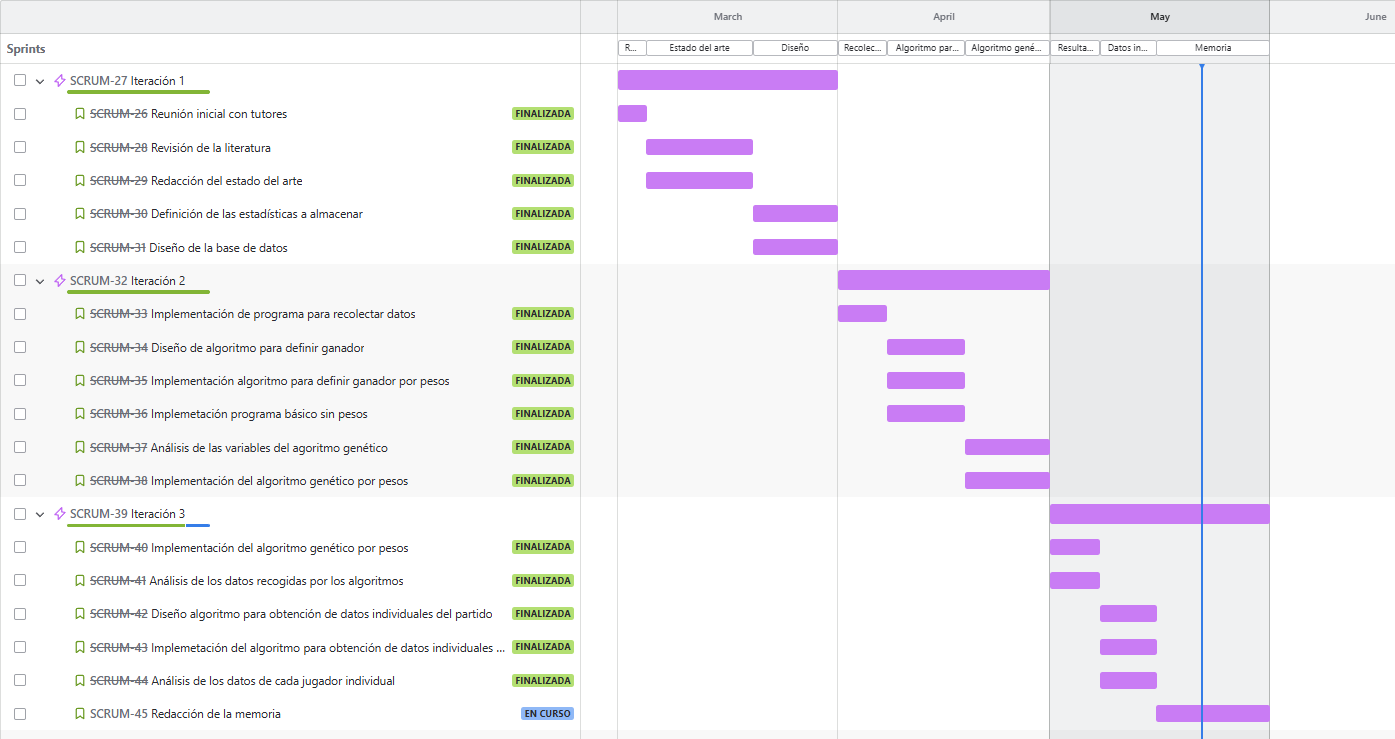
\includegraphics[width=\textheight, height=\textwidth, keepaspectratio]{plantilla-TFG-ETSIIT/doc/imagenes/Diagrama-Gantt.png}
    \end{sideways}
    \caption{Diagrama de Gantt del proyecto}
    \label{fig:imagen-ajustada}
\end{figure}

\section{Presupuesto}
\subsection*{Coste de personal}
Para este proyecto se necesita la contratación de un informático junior. Según \cite{sueldo-junior}, el sueldo de un programador junior en España es de 13.46 €/hora a lo que hay que
sumarle un aproximado 25\% por seguro médico, IRPF y demás impuestos. Durante este proyecto se ha trabajado durante 300 horas aproximadamente. También se necesita a un ingeniero en sistemas para mantener el servidor, según \cite{sueldo-sistemas} su sueldo medio es de 24.20 €/hora más un 25\% aproximado otra vez por impuestos, y ha trabajado 1 hora al día para verificar que todo estaba bien durante los 2 últimos meses del proyecto. También se va a prever 1 año más para dar soporte al proyecto y pueda mantenerse.

\begin{table}[h!]
\centering
\begin{tabular}{|c|c|c|c|}
\hline
\textbf{Descripción} & \textbf{Horas} & \textbf{€/hora} & \textbf{Coste(€)} \\
\hline
Programador junior & 300 & 13.46 & 4.038 \\
\hline
Ingeniero en sistemas & 425 & 24.20 & 10.285 \\
\hline
Total &  &  & 14.323 \\
\hline
\end{tabular}
\caption{Coste de personal}
\label{tab:ejemplo}
\end{table}

\subsection*{Coste de material}
En cuanto a hardware, se ha hecho de un portátil Lenovo Ideapad Gaming 3 cuyo coste de compra fue de 900 €. Hace 4 años que se compró, pero solo se va a usar durante un año, debido al mantenimiento del servidor. Simulando que se vaya a lanzar este proyecto de manera profesional, también se necesita el uso de un servidor con capacidad para albergar gran cantidad de datos. Se ha utilizado un servidor físico (HPE ProLiant MicroServer Gen10+) como plataforma para alojar la base de datos MongoDB, con un coste estimado de 775.98 €. Esto permite replicar un entorno profesional con servicios persistentes y seguros de gestión de datos.

En cuanto a software, se hace uso de MongoDB, Visual Studio, GitHub y Ubuntu; todos son gratuitos.

\begin{table}[h!]
\centering
\begin{tabular}{|c|c|c|c|c|}
\hline
\textbf{Descripción} & \textbf{Coste(€)} & \textbf{Años} & \textbf{Años usado} & \textbf{Coste(€)} \\
\hline
Portátil & 900 & 5 & 1 & 180 \\
\hline
Servidor & 775.98 & 1 & 1 & 775.98 \\
\hline
MongoDB & 0 & 1 & 1 & 0 \\
\hline
Visual Studio & 0 & 1 & 1 & 0 \\
\hline
GitHub & 0 & 1 & 1 & 0 \\
\hline
Ubuntu & 0 & 1 & 1 & 0 \\
\hline
Total &  & & & 955.98 \\
\hline
\end{tabular}
\caption{Coste de material}
\label{tab:ejemplo}
\end{table}

\subsection*{Costes indirectos}
Para los costes indirectos se estima un 10\% del gasto total del proyecto.
\begin{table}[h!]
\centering
\begin{tabular}{|c|c|c|c|}
\hline
\textbf{Descripción} & \textbf{Total} & \textbf{\%} & \textbf{Coste(€)} \\
\hline
Costes indirectos & 15.278,98 & 10 & 1.527,89 \\
\hline
Total &  &  & 16.806,87 \\
\hline
\end{tabular}
\caption{Costes indirectos}
\label{tab:ejemplo}
\end{table}

El coste total del proyecto sería de 16.806,87 €.

	% Análisis del problema
	% 1. Análisis de requisitos
	% 2. Análisis de las soluciones
	% 3. Solucion propuesta
	% 4. Análisis de seguridad
	\input{plantilla-TFG-ETSIIT/doc/secciones/04_analisis_diseño}

	% Implementación
	\chapter{Implementación}

\section{Datos}
Los datos utilizados en este trabajo han sido recopilados mediante técnicas de web scraping desde la página oficial de Sofascore \cite{Sofascore}. Para acceder a las estadísticas de un partido en dicha plataforma, basta con dirigirse a la sección ‘Estadísticas del jugador’, donde se despliega la información de todos los jugadores que participaron en el encuentro. Los mapas de calor, por su parte, se obtienen mediante una API que dispone de una función específica para tal fin.

Para incorporar los datos de un partido en la base de datos, es necesario proporcionar el nombre del jugador, el equipo, el rival correspondiente y la URL del partido; el sistema se encarga automáticamente de almacenar la información pertinente.

Dado que el código supera las cien líneas y está mayormente dedicado a ajustes relacionados con el proceso de scraping, se ha decidido no incluirlo íntegramente en este documento. No obstante, puede consultarse directamente en el repositorio disponible en GitHub.

\subsection{Mapas de calor}
Las estadísticas de los jugadores se almacenan como valores enteros o flotantes, reflejando directamente el valor cuantitativo de cada estadística (por ejemplo, 7 pases clave). Sin embargo, los mapas de calor se gestionan de manera distinta, ya que en ellos se registra una lista de pares de enteros que representan las coordenadas x e y correspondientes a las posiciones en el terreno de juego.

Para la representación gráfica del campo de fútbol se han utilizado las librerías matplotlib y mplsoccer, siendo esta última la encargada de dibujar el terreno de juego. A continuación, se muestra el código empleado para generar un campo vacío:


\begin{lstlisting}[language=Python, caption={Representación campo vacío}, label={lst:codigo-python}]
import matplotlib.pyplot as plt
from mplsoccer import Pitch

fig, ax = plt.subplots(figsize=(16, 9))
pitch = Pitch(pitch_type='opta')
pitch.draw(ax=ax)
plt.show()
\end{lstlisting}

La representación del campo vacío quedaría:

\begin{figure}[H]
    \centering
    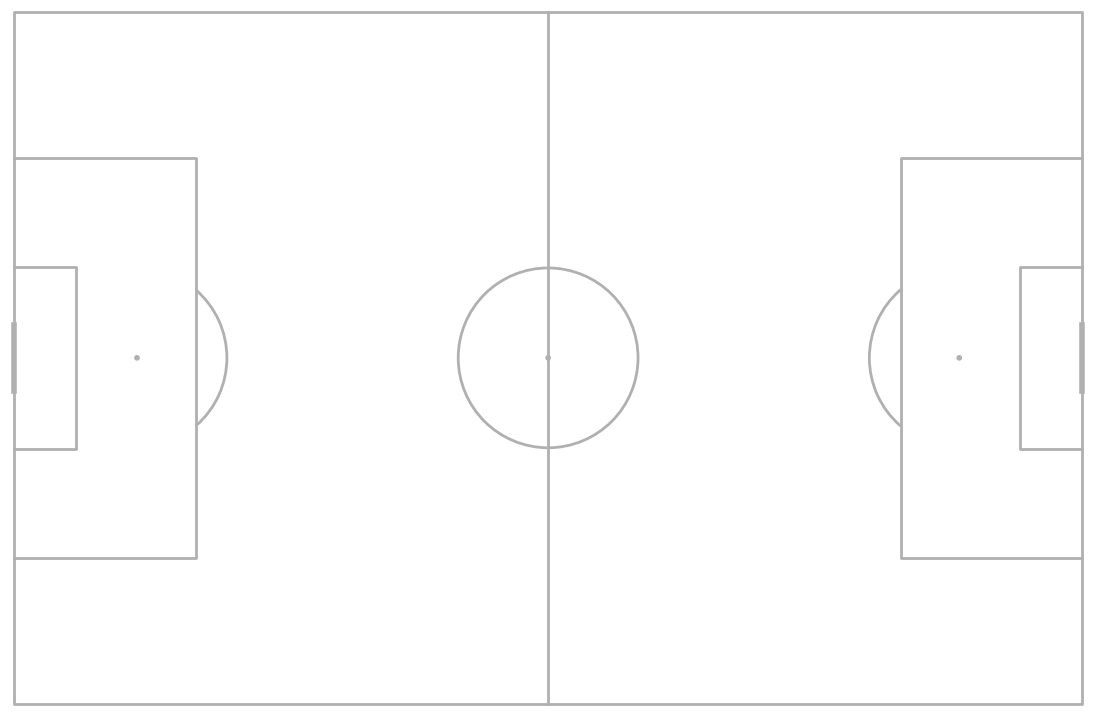
\includegraphics[width=0.7\textwidth]{plantilla-TFG-ETSIIT/doc/imagenes/Campo_vacio.png}
    \caption{Reprentación campo de fútbol}
    \label{fig:etiqueta-imagen}
\end{figure}

Es importante destacar que el punto (0, 0) corresponde a la esquina inferior izquierda del campo, mientras que el (99,99) se sitúa en la esquina superior derecha. Por ello, los mapas siempre se visualizarán de izquierda a derecha. Incluso cuando el jugador actúe como visitante, sus datos se ajustarán para mantener esta orientación constante, evitando así posibles confusiones.

Para representar el mapa de calor de un jugador específico, basta con extraer sus datos de la base de datos y graficarlos de manera similar a como se hizo anteriormente, rellenando el campo con las coordenadas correspondientes. A continuación, se presenta el código utilizado para ello:

\begin{lstlisting}[language=Python, caption={Mapa de calor de un futbolista}, label={lst:codigo-python}]

from pymongo import MongoClient
import pandas as pd
import matplotlib.pyplot as plt
from mplsoccer import Pitch
import warnings
from matplotlib.colors import LinearSegmentedColormap

warnings.filterwarnings("ignore")

# Conexion a mongoDB
cliente = MongoClient("mongodb://localhost:27017")
db = cliente["TFG"]
coleccion_jugadores = db["jugadores"]

# Buscar un jugador
jugador = coleccion_jugadores.find_one({"nombre": "Luis Milla", "equipo": "Getafe", "rival": "Villareal"})

# Verificar si se encontro el jugador
if jugador:

    mapa_calor_lista = jugador["mapa_calor"]
    mapa_calor_df = pd.DataFrame(mapa_calor_lista)
    colors = [(0, "white"), (0.5, "orange"), (1, "red")]
    custom_cmap = LinearSegmentedColormap.from_list("custom_cmap", colors)

    fig, ax = plt.subplots(figsize=(16, 9))

    pitch = Pitch(pitch_type='opta')
    pitch.draw(ax=ax)
    pitch.kdeplot(mapa_calor_df.x, mapa_calor_df.y, ax=ax,
                fill = True,
                levels=100,
                thresh=0.08,
                zorder=-1,
                bw_adjust=0.15,
                cmap="OrRd")

    # Anadir titulo personalizado
    nombre = jugador["nombre"]
    equipo = jugador["equipo"]
    rival = jugador["rival"]
    plt.title(f"Mapa de calor del jugador \"{nombre}\" del equipo \"{equipo}\", rival \"{rival}\"", fontsize=18)

    plt.show() 

else:
    print("Jugador no encontrado.")

\end{lstlisting}

Los ajustes en los valores utilizados para la representación del mapa de calor se han realizado manualmente, seleccionando aquellos que se consideraron más adecuados para una visualización clara y efectiva. A continuación, se ilustrará este proceso mediante ejemplos concretos de algunos jugadores.

El jugador Luis Milla, centrocampista del Getafe, presenta el siguiente mapa de calor correspondiente al partido disputado contra el Villarreal en la liga de la temporada 2024/2025:

\begin{figure}[H]
    \centering
    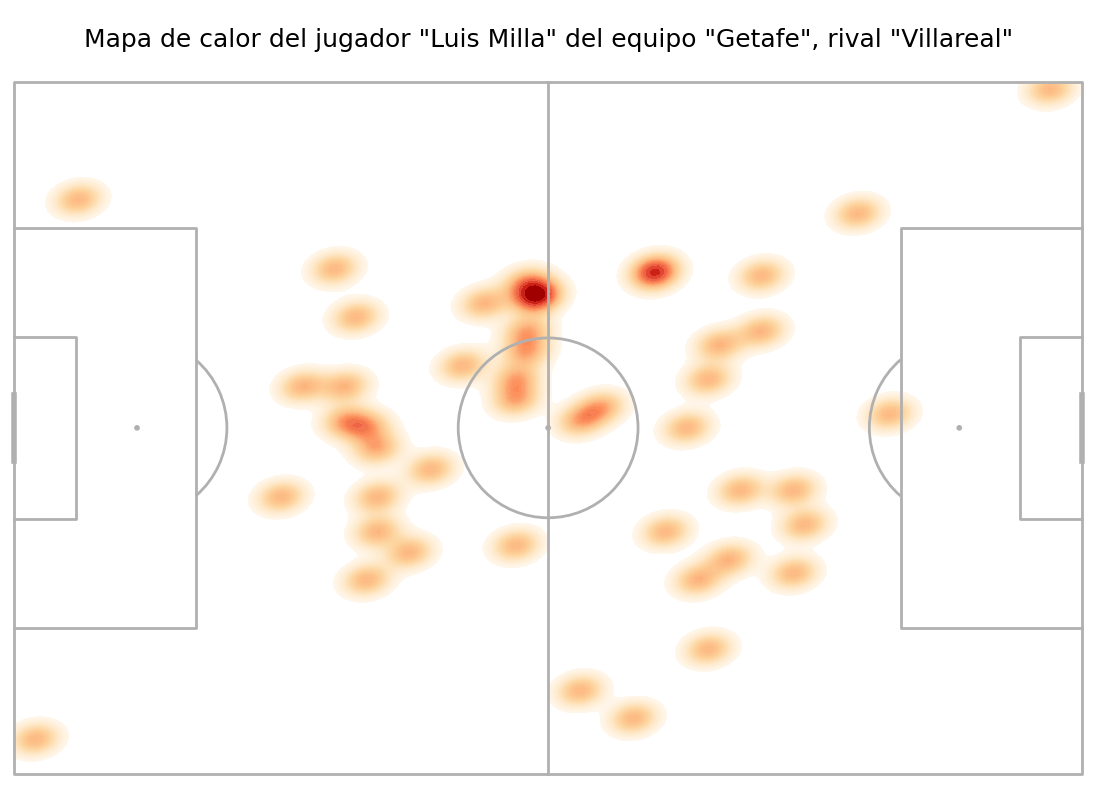
\includegraphics[width=0.7\textwidth]{plantilla-TFG-ETSIIT/doc/imagenes/Mapa_MC.png}
    \caption{Ejemplo representación de MC}
    \label{fig:etiqueta-imagen}
\end{figure}

Vamos a ver más ejemplos de otras posiciones distintas. El de un lateral derecho se vería algo así:

\begin{figure}[H]
    \centering
    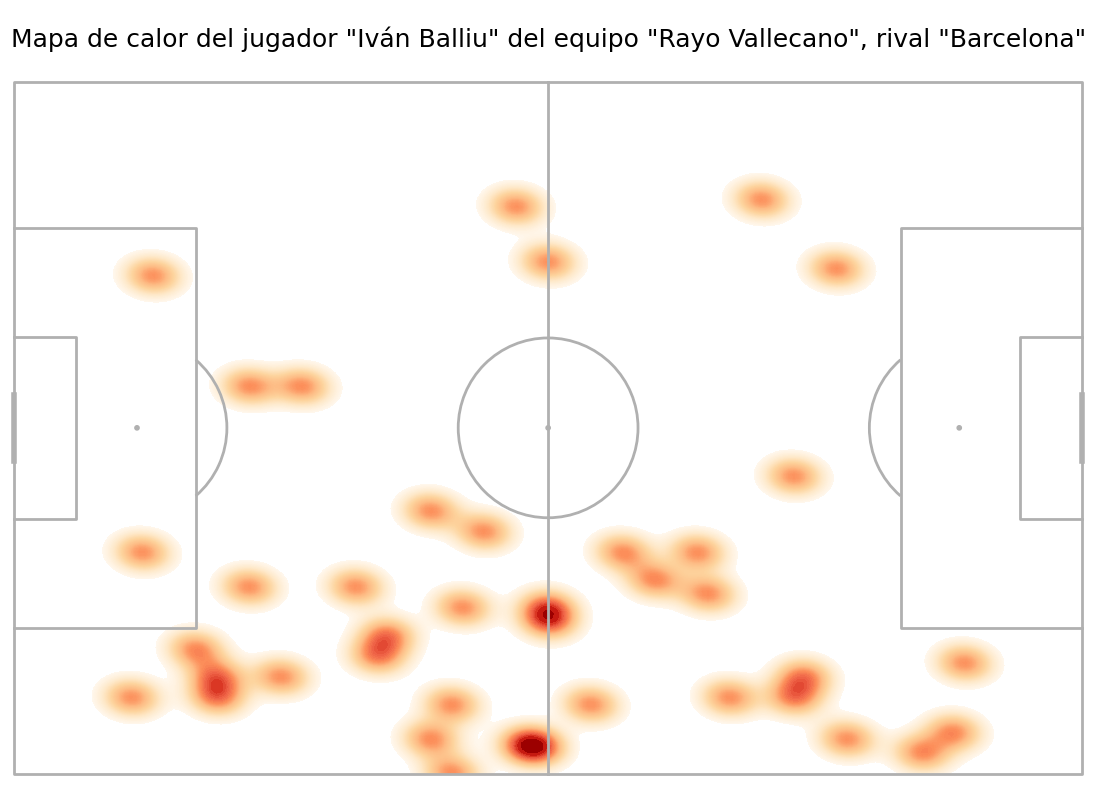
\includegraphics[width=0.7\textwidth]{plantilla-TFG-ETSIIT/doc/imagenes/Mapa_LD.png}
    \caption{Ejemplo representación de LD}
    \label{fig:etiqueta-imagen}
\end{figure}

Como se puede observar, al tratarse de un lateral derecho, su presencia predomina en la parte inferior del campo, teniendo en cuenta que la visualización del mapa se realiza de izquierda a derecha y de abajo hacia arriba.

Un ejemplo de un delantero extremo izquierdo se vería algo así:

\begin{figure}[H]
    \centering
    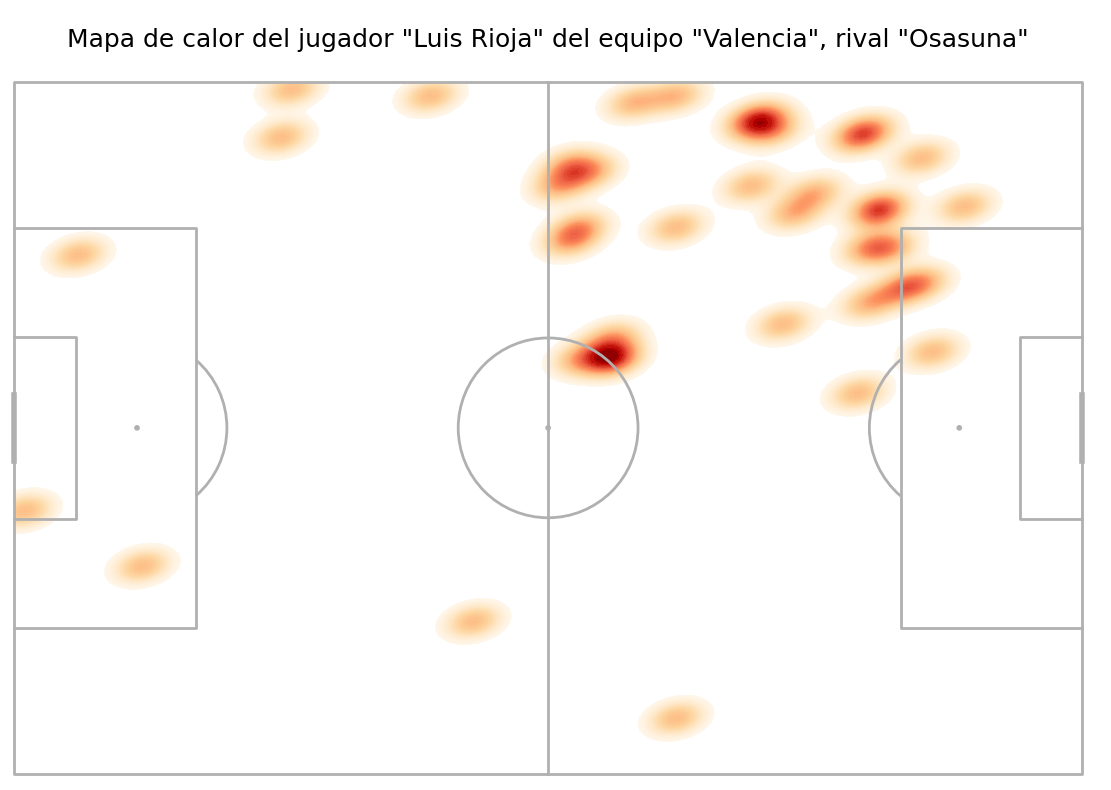
\includegraphics[width=0.7\textwidth]{plantilla-TFG-ETSIIT/doc/imagenes/Mapa_EI.png}
    \caption{Ejemplo representación de EI}
    \label{fig:etiqueta-imagen}
\end{figure}

Como se ve en la imagen, predomina principalmente la zona de arriba a la derecha que es la que pertenece al extremo izquierdo.

Por último, vamos a ver el mapa de calor de un portero, al que rara vez vamos a ver fuera del área.

\begin{figure}[H]
    \centering
    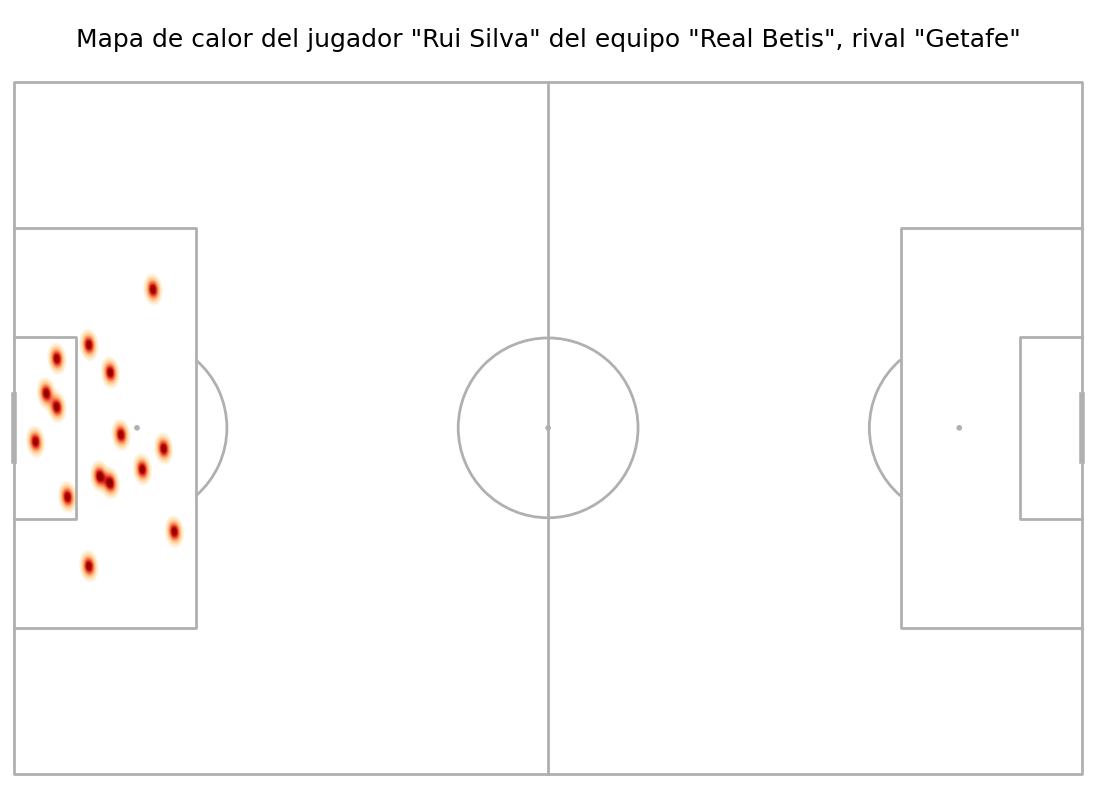
\includegraphics[width=0.7\textwidth]{plantilla-TFG-ETSIIT/doc/imagenes/Mapa_POR.png}
    \caption{Ejemplo representación de POR}
    \label{fig:etiqueta-imagen}
\end{figure}

Es importante destacar que los mapas de calor pueden presentar cierta aleatoriedad. Aunque los jugadores tienden a respetar sus posiciones habituales, en el transcurso de un partido pueden producirse situaciones inesperadas que los lleven a intervenir en otras zonas del campo, si bien estos casos son excepcionales. Por ejemplo, en el caso del extremo izquierdo, se observa que tocó el balón tres veces en su propia área, lo cual no es habitual y podría deberse a acciones defensivas en jugadas a balón parado. De manera similar, en el caso de Luis Milla, centrocampista, se aprecia que tocó el balón en las dos esquinas del campo, lo que sugiere que participó en la ejecución de saques de esquina.

\section{Algoritmo sin pesos}

Una vez obtenidos los datos de los jugadores almacenados en la base de datos, se procederá a explicar la implementación del algoritmo sin división por zonas, es decir, considerando únicamente las estadísticas individuales de los futbolistas sin segmentar el campo. No se han incluido todas las funciones debido a su extensión, pero sí se presenta la función principal del programa, que es la siguiente:

\begin{lstlisting}[language=Python, caption={Algoritmo sin zonas}, label={lst:codigo-python}]
if not JUGADORES_CACHE:
    inicializar_cache_jugadores()
#Bucle que recorre todos los partidos
for partido in coleccion_partidos.find():
    # Obtener jugadores
    jugadores1 = [jug for jug in JUGADORES_CACHE.values() if jug["equipo"] == partido["Local"] and jug["rival"] == partido["Visitante"] and jug["temporada"] == partido["Temporada"]]
    jugadores2 = [jug for jug in JUGADORES_CACHE.values() if jug["equipo"] == partido["Visitante"] and jug["rival"] == partido["Local"] and jug["temporada"] == partido["Temporada"]]
    
    maximos = calcularMaximos(jugadores1, jugadores2)

    suma_total_ofensiva_e1 = 0
    suma_total_defensiva_e1 = 0
    suma_total_ofensiva_e2 = 0
    suma_total_defensiva_e2 = 0

    for j in jugadores1:
        estadisticas_ofensivas = getEstadisticasOfensivas(j["_id"], maximos)
        estadisticas_defensivas = getEstadisticasDefensivas(j["_id"], maximos)
        suma_total_ofensiva_e1 += estadisticas_ofensivas
        suma_total_defensiva_e1 += estadisticas_defensivas
    for j in jugadores2:
        estadisticas_ofensivas = getEstadisticasOfensivas(j["_id"], maximos)
        estadisticas_defensivas = getEstadisticasDefensivas(j["_id"], maximos)
        suma_total_ofensiva_e2 += estadisticas_ofensivas
        suma_total_defensiva_e2 += estadisticas_defensivas
    
    total_e1 = suma_total_ofensiva_e1 - suma_total_defensiva_e2
    total_e2 = suma_total_ofensiva_e2 - suma_total_defensiva_e1

    resultado = total_e1 - total_e2

    if resultado > 2:
        resultado = "local"
    elif resultado < -2:
        resultado = "visitante"
    else:
        resultado = "empate"
\end{lstlisting}

Como se explicó anteriormente, este enfoque se basa únicamente en la sumatoria de las estadísticas normalizadas de todos los jugadores de cada equipo. El equipo que obtenga una puntuación total más alta será considerado el ganador.

En este caso, el umbral de decisión, fijado en el valor 2, se ha definido manualmente, ya que se trata de un algoritmo sencillo en el que no se ha aplicado ninguna técnica de \textit{machine learning}.

Las funciones 'getEstadisticasOfensivas' y 'getEstadisticasDefensivas' recorren los datos de cada jugador y extraen únicamente las estadísticas correspondientes, que han sido previamente normalizadas en un rango de 0 a 1. En esta escala, un valor de 1 representa la mejor ejecución de esa estadística dentro del partido, mientras que un valor de 0 indica el rendimiento más bajo registrado.
Los resultados de la ejecución de este algoritmo se pueden ver en la sección 6.1 en el siguiente capítulo.

\section{Algoritmo con pesos}
A continuación, se procede a la implementación del algoritmo descrito en el capítulo anterior. Tal como se indicó, el enfoque consiste en dividir el terreno de juego en 24 zonas, asignando a cada una un peso determinado en función de su relevancia para el análisis.

La distribución del campo en zonas se ha diseñado de forma que permita una evaluación más precisa del impacto de cada jugador en áreas específicas del terreno de juego. Esta segmentación facilita una interpretación más detallada del rendimiento colectivo e individual durante el partido.

La división utilizada es la siguiente:

\begin{figure}[H]
    \centering
    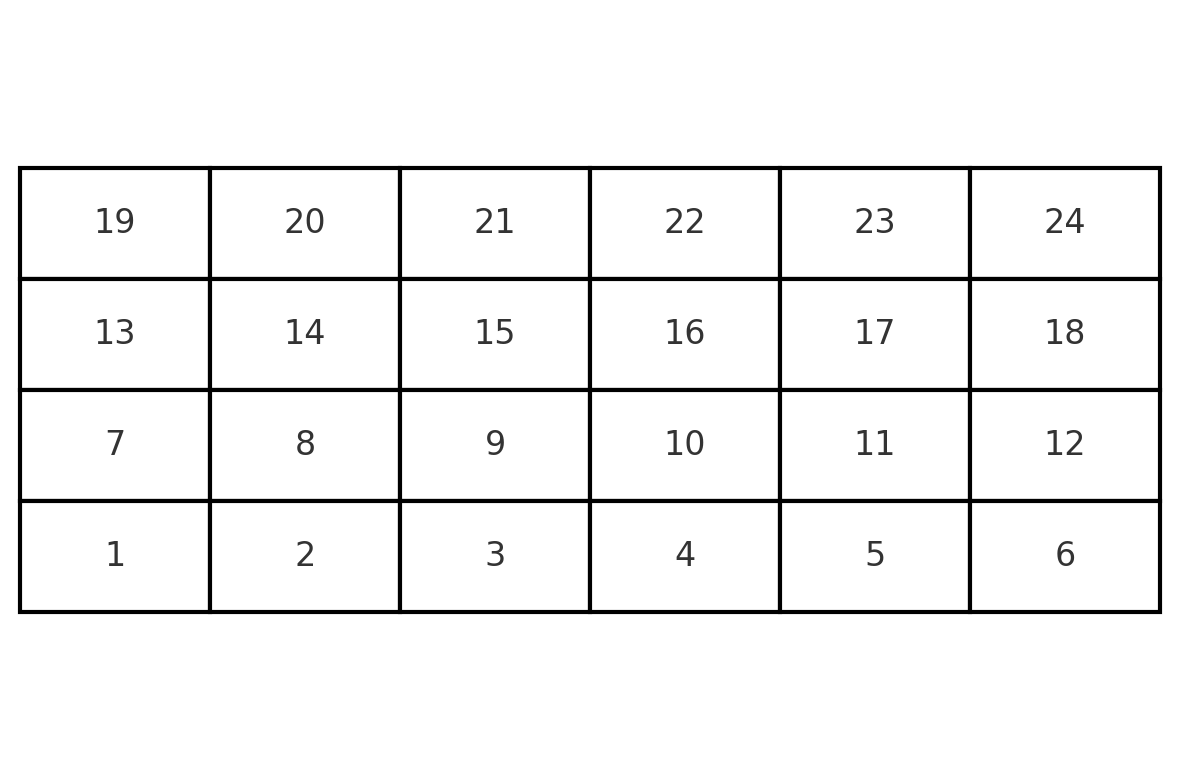
\includegraphics[width=0.6\textwidth]{plantilla-TFG-ETSIIT/doc/imagenes/Zonas_campo.png}
    \caption{Distribución en zonas del campo}
    \label{fig:etiqueta-imagen}
\end{figure}

Al igual que en los apartados anteriores, el campo se representa orientado de izquierda a derecha, de forma que las zonas 6, 12, 18 y 24 corresponden a las áreas de máximo ataque, mientras que las zonas 1, 7, 13 y 19 representan las zonas más defensivas.

Para este enfoque inicial, se han definido dos vectores de pesos: uno destinado a las estadísticas constructivas (ofensivas) y otro a las destructivas (defensivas). No obstante, en la implementación del código, ambos se gestionan como un único vector para simplificar su tratamiento.

La razón de esta separación conceptual es garantizar una evaluación adecuada del rendimiento en función del tipo de estadística. Por ejemplo, no tendría sentido asignar un peso elevado a una acción defensiva en una zona ofensiva, ya que su impacto real en el juego sería escaso. Así, el vector de ataque incrementa sus valores a medida que las zonas se aproximan al área rival, mientras que el vector de defensa lo hace en dirección contraria, aumentando su importancia conforme se acerca a la propia portería.

De este modo, se definen los siguientes vectores iniciales. A continuación, se muestra el correspondiente a las estadísticas ofensivas:

\begin{figure}[H]
    \centering
    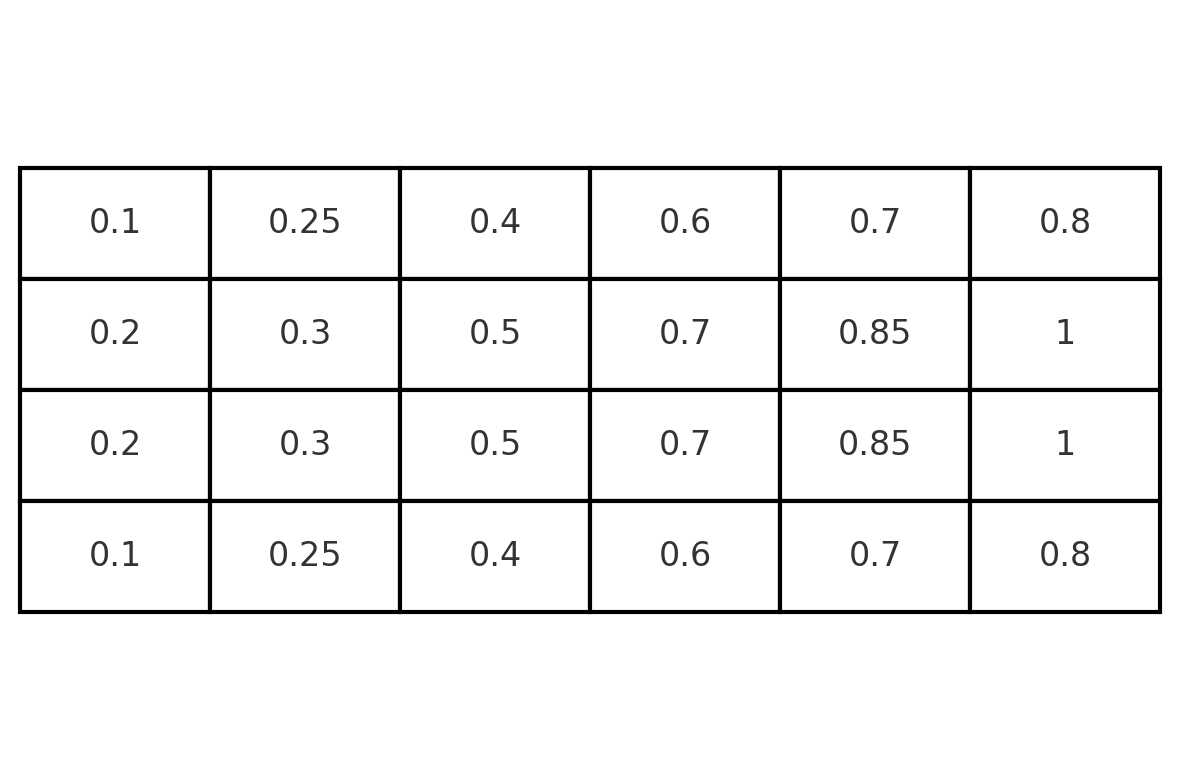
\includegraphics[width=0.8\textwidth]{plantilla-TFG-ETSIIT/doc/imagenes/Pesos_ini_ataque.png}
    \caption{Vector inicial de ataque}
    \label{fig:etiqueta-imagen}
\end{figure}

Y el vector inicial para las estadísticas defensivas:

\begin{figure}[H]
    \centering
    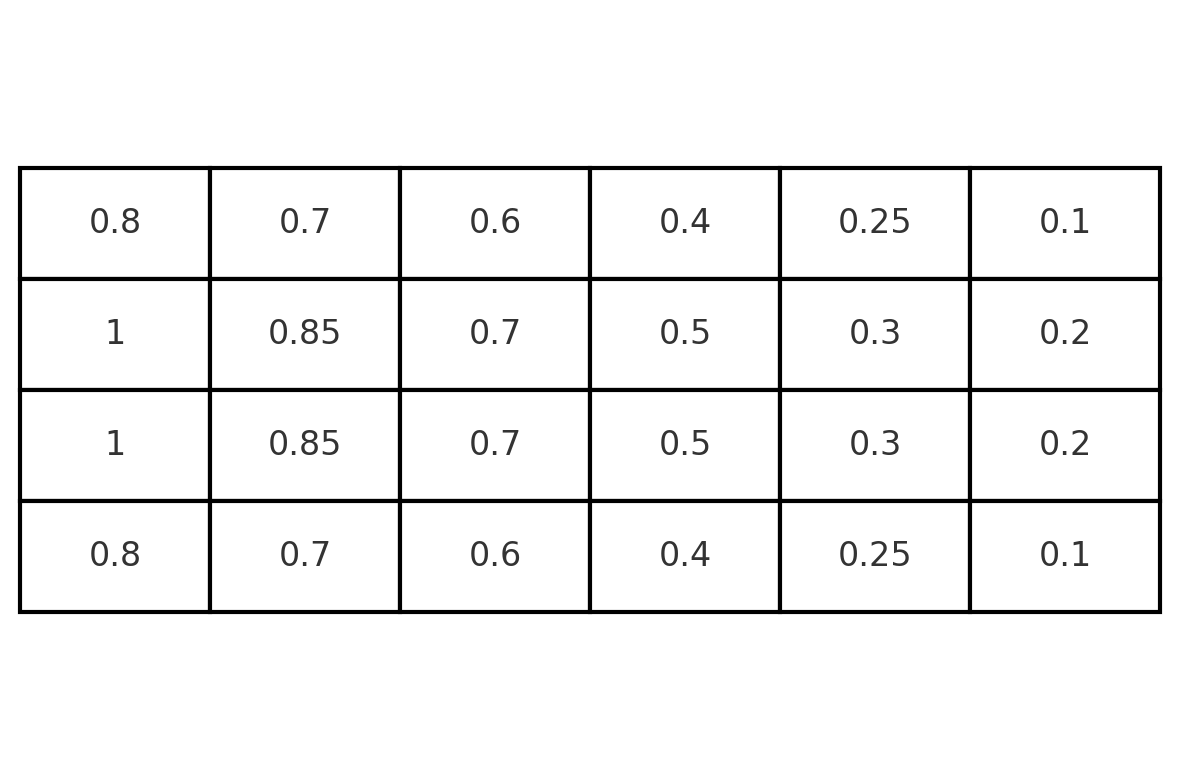
\includegraphics[width=0.8\textwidth]{plantilla-TFG-ETSIIT/doc/imagenes/Pesos_ini_defensa.png}
    \caption{Vector inicial de defensa}
    \label{fig:etiqueta-imagen}
\end{figure}

Una vez definidos los pesos correspondientes a cada zona del terreno de juego, se procede a la implementación del algoritmo. El primer paso consiste en inicializar los datos de los jugadores que han participado en el partido en cuestión. Estos datos serán la base para calcular las estadísticas ponderadas por zona, necesarias para determinar el rendimiento colectivo e individual a lo largo del campo.

\begin{lstlisting}[language=Python, caption={Inicialización datos}, label={lst:codigo-python}]
def calcula_zonas(local, visitante, temporada, corte=2):
    if not JUGADORES_CACHE:
        inicializar_cache_jugadores()

    # Obtener el partido
    partido = resultados.find_one({"Local": local, "Visitante": visitante, "Temporada": temporada})
    if not partido:
        raise ValueError(f"No se encontro el partido entre {local} y {visitante} en la temporada {temporada}.")

    jugadores1 = [jug for jug in JUGADORES_CACHE.values() if jug["equipo"] == local and jug["rival"] == visitante and jug["temporada"] == temporada]
    jugadores2 = [jug for jug in JUGADORES_CACHE.values() if jug["equipo"] == visitante and jug["rival"] == local and jug["temporada"] == temporada]
    
    preprocesar_mapa_calor(jugadores1)
    preprocesar_mapa_calor(jugadores2)

    maximos = calcularMaximos(jugadores1, jugadores2)

\end{lstlisting}

Primero se inicializan los jugadores en la caché, esto se hace para disminuir las consultas a la base de datos. De esta forma se buscan todos los jugadores una vez y se guardan en una variable llamada $\text{JUGADORES\_CACHE}$.

A continuación, se realiza una consulta para localizar el partido específico que se desea analizar, y se inicializan las variables correspondientes con los jugadores involucrados. Una vez hecho esto, se procesan los mapas de calor de cada futbolista, calculando el porcentaje de tiempo que han permanecido en cada una de las zonas del campo.

Finalmente, se determinan los valores máximos alcanzados por cada estadística entre todos los jugadores del encuentro. Estos valores se almacenan en variables locales y servirán para normalizar las estadísticas individuales, permitiendo una comparación justa y coherente entre todos los participantes.

\begin{lstlisting}[language=Python, caption={Procesamiento de cada zona}, label={lst:codigo-python}]
for z in zonas[:-1]:
        suma_total_ofensiva_e1 = 0
        suma_total_defensiva_e1 = 0
        suma_total_ofensiva_e2 = 0
        suma_total_defensiva_e2 = 0
        for j in jugadores1:
            porc = calcularPorcentaje(j, z)
            if porc != 0:
                estadisticas_ofensivas = getEstadisticasOfensivas(j["_id"], maximos) * porc
                estadisticas_defensivas = getEstadisticasDefensivas(j["_id"], maximos) * porc
                suma_total_ofensiva_e1 += estadisticas_ofensivas
                suma_total_defensiva_e1 += estadisticas_defensivas

        for j2 in jugadores2:
            porc = calcularPorcentaje(j2, z)
            if porc != 0:
                estadisticas_ofensivas = getEstadisticasOfensivas(j2["_id"], maximos) * porc
                estadisticas_defensivas = getEstadisticasDefensivas(j2["_id"], maximos) * porc
                suma_total_ofensiva_e2 += estadisticas_ofensivas
                suma_total_defensiva_e2 += estadisticas_defensivas

\end{lstlisting}

El algoritmo implementado funciona de la siguiente manera: para cada una de las zonas del terreno de juego, se recorren los jugadores de ambos equipos. Por cada jugador, se extraen sus estadísticas correspondientes, que ya han sido previamente normalizadas. Estas estadísticas se ponderan multiplicándolas por el porcentaje de influencia del jugador en la zona concreta, según lo indica su mapa de calor.

De esta forma, se obtiene una medida ajustada del impacto real de cada futbolista en cada zona del campo. Las estadísticas ponderadas se suman directamente al total correspondiente de su equipo, permitiendo así calcular una puntuación global que refleja el rendimiento colectivo en función del posicionamiento y la actividad individual de cada jugador.

\begin{lstlisting}[language=Python, caption={Procesamiento de cada zona}, label={lst:codigo-python}]
    zonas_valores_e1[z-1] = (suma_total_ofensiva_e1*zonas_coeficientes[z-1] - suma_total_defensiva_e2*zonas_coeficientes[z-1+24])
    
    zonas_valores_e2[z-1] = (suma_total_ofensiva_e2*zonas_coeficientes[z-1] - suma_total_defensiva_e1*zonas_coeficientes[z-1+24])
    
    total_rival[z-1] = (suma_total_ofensiva_e2*zonas_coeficientes[z-1] + suma_total_defensiva_e1*zonas_coeficientes[z-1+24])

suma_total = sum(zonas_valores_e1) - sum(zonas_valores_e2)

if suma_total > corte:
    return 1
elif suma_total < -corte:
    return 2
else:
    return 0

\end{lstlisting}

Una vez calculados los valores totales ofensivos y defensivos de cada equipo en cada zona del campo, el siguiente paso consiste en ponderarlos utilizando los pesos previamente definidos para cada zona. Es decir, se multiplica el valor obtenido en cada zona por su peso correspondiente, según si se trata de acciones ofensivas o defensivas.

Finalmente, se suman los resultados ponderados de todas las zonas y se comparan los totales obtenidos por ambos equipos. En función de estos valores globales, se determina el ganador del encuentro: vence el equipo con la mayor puntuación, o se declara empate si los resultados son equivalentes. Se puede ver el resultado de la ejecución de este algoritmo en el siguiente capítulo.

\section{Algoritmo genético}

Para implementar el algoritmo genético, se ha definido un único vector que representa tanto las ponderaciones ofensivas como defensivas, considerando que ambas forman parte del mismo individuo dentro de la población. Este vector tiene una longitud de 48 elementos, ya que el terreno de juego se ha dividido en 24 zonas y se asigna un peso específico a cada una, tanto para las acciones ofensivas como para las defensivas. Cada uno de los valores del vector se encuentra en el rango [0, 1], representando así la influencia relativa de cada zona en el rendimiento global del equipo.

\subsection*{Función de evaluación}
Para evaluar la calidad de un individuo, se utiliza la función evaluar\_vector, que recibe como argumento el vector de coeficientes y lo aplica a todos los partidos almacenados en la base de datos. Esta función calcula el porcentaje de aciertos que obtiene el vector al predecir los resultados. Cuanto mayor sea este porcentaje, mayor será la calidad y precisión del individuo dentro del algoritmo genético.

\subsection*{Operadores genéticos}

Para la selección se ha optado por el método de selección por torneo. Según lo expuesto por Miller y Goldberg en \cite{algoritmo_genetico}, esta técnica es muy precisa, ya que combina aleatoriedad con la elección de los mejores individuos, lo que permite mantener diversidad genética mientras se favorece la supervivencia de las soluciones más aptas.

\begin{lstlisting}[language=Python, caption={Selección por torneo}, label={lst:codigo-python}]
toolbox.register("select", tools.selTournament)
def algoritmo_genetico():
    ...
    offspring = toolbox.select(poblacion, len(poblacion) - 1,TAMANO_TORNEO)

\end{lstlisting}

El cruzamiento se realiza con una probabilidad muy alta para fomentar la diversidad entre los individuos. En las distintas ejecuciones realizadas, la tasa de cruzamiento ha sido de 0.9 o 1. Una vez seleccionados los dos vectores que se cruzarán, el proceso se lleva a cabo mediante un cruzamiento uniforme, donde cada gen tiene una probabilidad del 50\% de ser intercambiado entre ambos padres.

\begin{lstlisting}[language=Python, caption={Cruzamiento}, label={lst:codigo-python}]
toolbox.register("mate", tools.cxUniform, indpb=0.5)

def algoritmo_genetico():
        ...
        for i in range(1, len(offspring), 2):
            if np.random.rand() < TASA_CRUZAMIENTO:
                toolbox.mate(offspring[i-1], offspring[i])
\end{lstlisting}

La mutación se aplica con una probabilidad de 1 / (tamaño de población) a cada gen, es decir, a cada elemento del vector de pesos.
    
\begin{lstlisting}[language=Python, caption={Función mutación}, label={lst:codigo-python}]
def mutacion_uniforme_flotante(individuo, low=0.0, up=1.0, indpb = INDPB_MUTACION):
    for i in range(len(individuo)):
        if np.random.rand() < indpb:
            individuo[i] = np.random.uniform(low, up)
    return individuo,
\end{lstlisting}

\begin{lstlisting}[language=Python, caption={aplicación función mutación}, label={lst:codigo-python}]
toolbox.register("mutate", mutacion_uniforme_flotante, low=0.0, up=1.0, indpb=INDPB_MUTACION)

def algoritmo_genetico():
    ...
    for ind in offspring:
            toolbox.mutate(ind)
\end{lstlisting}

\subsection*{Elitismo}
Para garantizar que la mejor solución no se pierda durante el proceso evolutivo, se implementa elitismo, el cual conserva al mejor individuo de cada generación.

\begin{lstlisting}[language=Python, caption={Implementación elitismo}, label={lst:codigo-python}]
def algoritmo_genetico():
    ...
    elite = tools.selBest(poblacion, k=1)
    poblacion[:] = elite + offspring

\end{lstlisting}

\section{Algoritmo genético con $\delta$}
Con el objetivo de mejorar la precisión de la predicción, se ha decidido incluir en el vector de pesos el parámetro $\delta$, que representa el umbral de corte para decidir el resultado: si gana un equipo, el otro o si hay empate. Hasta ahora, este valor se había fijado manualmente en 2, es decir, si:

\begin{itemize}
    \item $Score global > 2$, gana local
    \item $Score global < -2$, gana visitante
    \item empate en caso contrario
\end{itemize}

El algoritmo genético, además de optimizar los vectores de ponderaciones para las zonas de ataque y defensa del campo, incluirá ahora la variable $\delta$ dentro del vector de parámetros a ajustar. La configuración del algoritmo es la misma que la descrita anteriormente, salvo por la tasa de mutación, que se ha ajustado a 1 / 49 debido al incremento en la longitud del vector. El propósito es comparar distintas técnicas para evaluar cuál ofrece un mejor equilibrio entre precisión y coste computacional.

Se probarán los mismos valores que en las ejecuciones anteriores, realizando un total de 5 repeticiones para cada combinación y calculando la media y la desviación típica de los resultados obtenidos.


	% Trabajos futuros

        \chapter{Análisis de resultados}

Este capítulo presenta un estudio secuencial de los resultados, comenzando por la ejecución y evaluación de los algoritmos base que establecen los parámetros iniciales del modelo. En primer término, se implementa y analiza el algoritmo sin ponderación de zonas, que ofrece una línea base de rendimiento al tratar todas las áreas del campo con igual importancia. A continuación, se examina el comportamiento del algoritmo con ponderación uniforme, donde se asignan pesos estándar a cada zona, permitiendo una primera aproximación a las diferencias espaciales.

Una vez establecidas estas referencias iniciales, la investigación avanza hacia un análisis más granular. Se estudia el rendimiento colectivo de los equipos examinando su influencia diferencial en las distintas zonas del campo, revelando patrones espaciales asociados al éxito deportivo. Este enfoque macro complementa el posterior análisis individual de jugadores mediante mapas de calor, que cuantifican la participación y efectividad de cada futbolista en áreas específicas.

La fase culminante aplica dos algoritmos genéticos que optimizan dinámicamente la ponderación zonal, contrastando sus resultados con los modelos base iniciales. Esta estructura metodológica, de lo general a lo particular, y de los modelos simples a los complejos, permite una validación rigurosa del sistema, demostrando cómo la ponderación inteligente de zonas mejora la capacidad predictiva respecto a los enfoques no ponderados.

El capítulo no solo compara la eficacia de cada método, sino que revela computacionalmente qué regiones del campo resultan más decisivas, proporcionando insights valiosos para la toma de decisiones técnicas. Esta progresión analítica garantiza una comprensión profunda de los factores espaciales que influyen en el rendimiento futbolístico.

\section{Algoritmo sin pesos}
La ejecución del algoritmo sin zonas, explicado en el capítulo anterior, es la siguiente:

\begin{figure}[H]
    \centering
    
\includegraphics[width=1.0\textwidth]{plantilla-TFG-ETSIIT/doc/imagenes/Ejecucion_simple.png}
    \caption{Ejecución algoritmo sin pesos}
    \label{fig:etiqueta-imagen}
\end{figure}

Al ejecutar el modelo sobre todos los partidos de la base de datos, se obtiene una precisión del 36,14\%, un valor relativamente bajo si se considera que existen únicamente tres posibles resultados en un partido: victoria local, victoria visitante o empate. Esto implica que la predicción se aproxima al azar, donde cada resultado tendría una probabilidad cercana al 33,3\%.


\section{Algoritmo con pesos}
La ejecución del algoritmo con zonas, el cual también ha sido explicado en el capítulo anterior, muestra:

\begin{figure}[H]
    \centering
    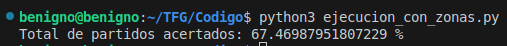
\includegraphics[width=1.0\textwidth]{plantilla-TFG-ETSIIT/doc/imagenes/Ejecucion_con_zonas.png}
    \caption{Ejecución algoritmo con pesos}
    \label{fig:etiqueta-imagen}
\end{figure}

Al ejecutar este algoritmo sobre todos los partidos disponibles en la base de datos, se obtiene una precisión del 67,47\%, una mejora significativa respecto a enfoques anteriores. Aunque este porcentaje ya puede considerarse aceptable dentro del contexto de la predicción de resultados en fútbol, aún existe margen de mejora, especialmente mediante el ajuste fino de los pesos y la incorporación de técnicas más avanzadas.

\section{Rendimiento de los equipos}
Una funcionalidad adicional incorporada al algoritmo con pesos es que permite visualizar el dominio territorial de cada equipo en el terreno de juego, a partir de la suma total de acciones realizadas en cada zona. Esta representación se genera mediante la función 'representar\_mapa', que recibe como argumentos dos vectores correspondientes a la sumatoria total de cada equipo en las 24 zonas del campo.

La función produce un mapa dividido en dichas zonas, coloreando en rojo aquellas en las que predomina el equipo 1 y en azul las dominadas por el equipo 2. Además, se tiene en cuenta la simetría del campo para mantener una visualización coherente: independientemente de si el equipo es local o visitante, sus estadísticas se ajustan para que ambos ataquen siempre de izquierda a derecha en la representación. De este modo, si el equipo visitante tiene mayor presencia ofensiva, dicha superioridad se visualizará en las zonas de ataque habituales, pero con el color azul que lo identifica.

A continuación, se muestra un ejemplo aplicado al partido Villarreal - Las Palmas correspondiente a la temporada 2024/2025 de la liga española:

\begin{figure}[H]
    \centering
    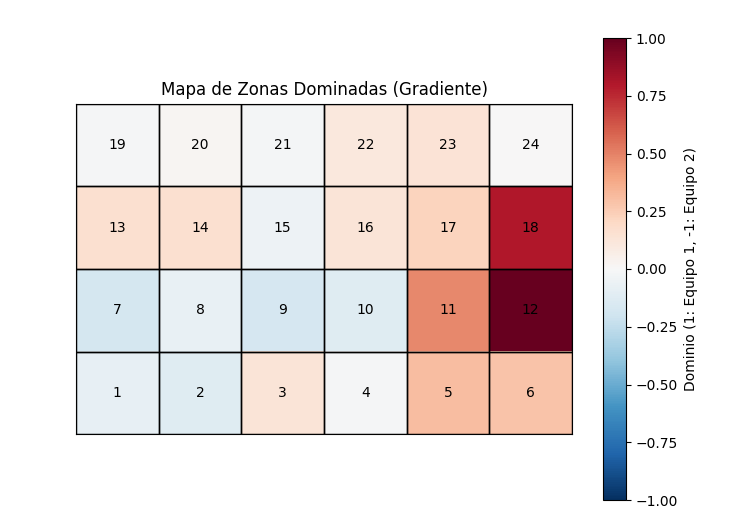
\includegraphics[width=0.6\textwidth]{plantilla-TFG-ETSIIT/doc/imagenes/Local_zonas_equipos.png}
    \caption{Mapa de zonas resultante del Villareal - Las Palmas}
    \label{fig:etiqueta-imagen}
\end{figure}

Como se puede observar en el mapa, el equipo local, el Villarreal, dominó claramente las zonas de ataque, especialmente aquellas más próximas a la portería rival. Este comportamiento es coherente con el resultado final del encuentro, que terminó con una victoria del Villarreal por 3-1. Este tipo de representación permite a los entrenadores obtener conclusiones tácticas relevantes: por ejemplo, se aprecia que el equipo visitante recibió una mayor presión por la banda derecha, incluso hasta la línea de fondo, lo que podría indicar la necesidad de reforzar la defensa en esa zona.
Del mismo modo, el cuerpo técnico del Villarreal podría interpretar este mapa como una confirmación del buen rendimiento colectivo, ya que su equipo apenas fue superado en ninguna zona del campo. En aquellos sectores donde el rival sí logró cierta presencia, las diferencias son mínimas, lo que podría considerarse como un equilibrio más que una desventaja.

A continuación, se analiza un ejemplo del Getafe - Las Palmas de la temporada 2024/2025 de la liga española, en el que el equipo visitante resultó vencedor:

\begin{figure}[H]
    \centering
    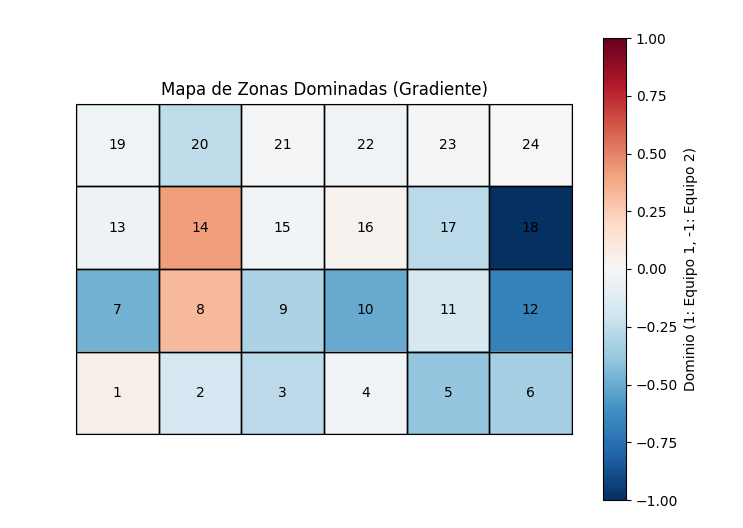
\includegraphics[width=0.7\textwidth]{plantilla-TFG-ETSIIT/doc/imagenes/Visitante_zonas_equipo.png}
    \caption{Mapa de zonas resultante del Getafe - Las Palmas}
    \label{fig:etiqueta-imagen}
\end{figure}

En este caso, puede apreciarse que el equipo visitante, representado en color azul, ha dominado en prácticamente todas las zonas del campo, con excepción de las dos zonas centrales de defensa. Esta distribución sugiere que el equipo local centró sus esfuerzos principalmente en tareas defensivas, concentrando su actividad en dichas áreas con el objetivo de contener los ataques rivales. Sin embargo, el amplio control territorial del equipo visitante indica un dominio generalizado del juego, lo que permite inferir que, a pesar de la resistencia defensiva local, no se logró frenar la ofensiva sostenida del adversario.

A continuación, se muestra un ejemplo correspondiente a un partido que finalizó en empate:

\begin{figure}[H]
    \centering
    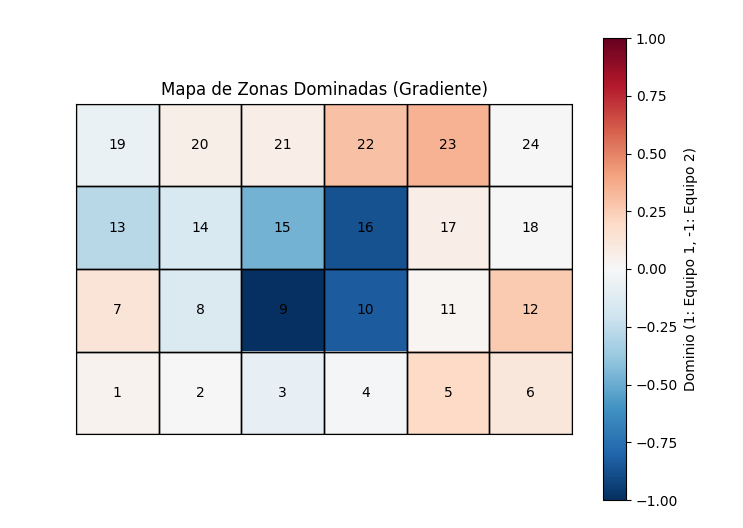
\includegraphics[width=0.7\textwidth]{plantilla-TFG-ETSIIT/doc/imagenes/Empate_zonas_equipos.png}
    \caption{Mapa de zonas resultante del Las Palmas - Sevilla}
    \label{fig:etiqueta-imagen}
\end{figure}

En el ejemplo correspondiente al encuentro entre Las Palmas y Sevilla, disputado durante la temporada 2024/2025 de la liga española, se observa que ninguno de los dos equipos logró dominar con claridad las zonas de ataque del adversario. No obstante, el equipo local mostró un mayor control en el centro del campo, aunque esta superioridad no fue suficiente para traducirse en una victoria.

Este tipo de visualización ofrece información valiosa para los entrenadores, ya que permite identificar con precisión las zonas del terreno donde el equipo necesita mejorar. A partir del análisis espacial del rendimiento, es posible extraer conclusiones tácticas relevantes y establecer líneas de actuación concretas de cara a futuros partidos.

\section{Rendimiento individual de cada futbolista}
En el análisis futbolístico, no solo es relevante estudiar el rendimiento colectivo del equipo, sino también el desempeño individual de cada jugador. Al igual que es posible acceder a la suma de acciones realizadas por el conjunto en cada zona del campo, este mismo análisis puede aplicarse a nivel individual. Esta perspectiva permite identificar qué futbolistas han tenido una participación más determinante durante el partido y cuáles han contribuido en menor medida.

La evaluación se basa en comparar la aportación del jugador en cada zona del campo con la suma total de las acciones del equipo en esa misma área. Al igual que en representaciones anteriores, los mapas se muestran siempre con el equipo atacando de derecha a izquierda, independientemente de si actúa como local o visitante. Para cada zona, si un jugador presenta una estadística igual o ligeramente inferior (hasta 0.2 puntos) respecto al total del equipo rival, se considera que ha tenido un papel relevante, aunque no diferencial, y se representa con un tono rojo claro. En cambio, si el jugador supera en una zona concreta la suma de las estadísticas del rival, dicha área se representa con un gradiente de color rojo, siendo más intenso en las zonas donde su impacto ha sido mayor. Todos los valores donde se ha sido predominante han sido normalizados en un rango de 0.0 a 0.1, excluyéndose de la normalización aquellos inferiores a -0.2, ya que no se consideran suficientemente significativos y se representan en el mapa de color blanco. 

A continuación, se muestran algunos mapas de calor correspondientes al encuentro entre Real Madrid F y Valencia F, perteneciente a la primera división femenina de España, con el objetivo de ilustrar esta metodología aplicada al análisis individual.

\begin{figure}[H]
    \centering
    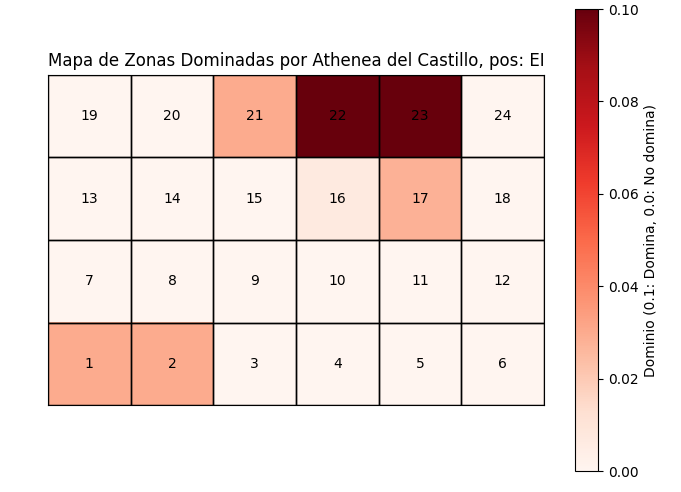
\includegraphics[width=0.7\textwidth]{plantilla-TFG-ETSIIT/doc/imagenes/futbolista_mapa_1.png}
    \caption{Mapa de influencia de Athenea de Castillo}
    \label{fig:etiqueta-imagen}
\end{figure}

Como se puede observar, esta futbolista que juega como extrema izquierda, dominó en las áreas relativas a su posición (17, 21, 22, 23), por lo que se puede deducir que fue capaz de desestabilizar a la defensa rival en esas zonas.

A continuación, se presenta el mapa de calor de la extrema izquierda que entró como sustituta de la futbolista que acabamos de ver:

\begin{figure}[H]
    \centering
    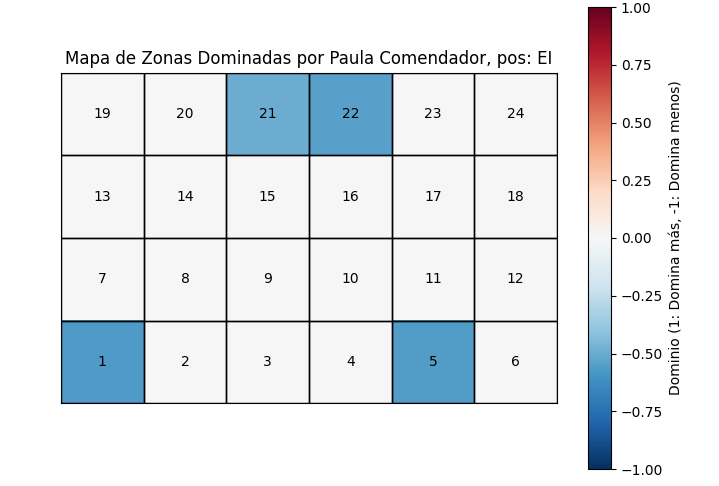
\includegraphics[width=0.7\textwidth]{plantilla-TFG-ETSIIT/doc/imagenes/Futbolista_mapa_3.png}
    \caption{Mapa de influencia de Paula Comendador}
    \label{fig:etiqueta-imagen}
\end{figure}

Como se observa, esta futbolista no fue tan dominante en las áreas relativas a su posición, de hecho, la extrema titular domina en más zonas y con más intensidad que ella. Esta información puede ser de gran utilidad para el entrenador a la hora de comparar futbolistas y tomar decisiones respecto a las alineaciones.

A continuación, se presenta el mapa de calor de una jugadora que desempeña el rol de lateral derecha, recordemos que la zonas en rojo reflejan que las estadísticas de la futbolista en el partido superan en su totalidad al del equipo rival en esa zona:

\begin{figure}[H]
    \centering
    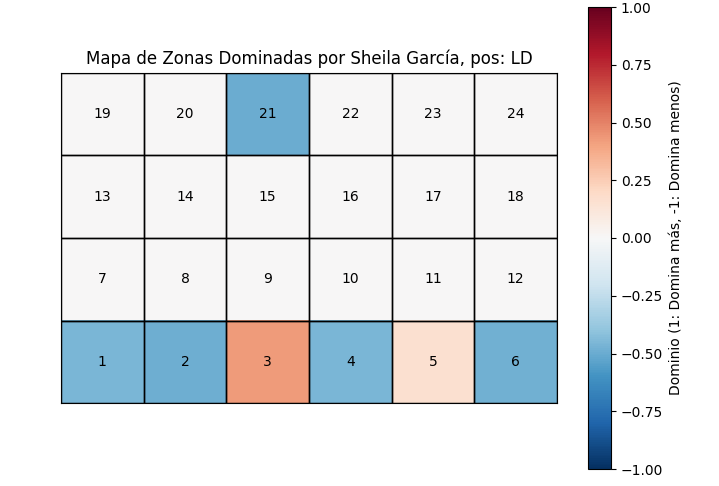
\includegraphics[width=0.7\textwidth]{plantilla-TFG-ETSIIT/doc/imagenes/Futbolista_mapa_2.png}
    \caption{Mapa de influencia de Sheila García}
    \label{fig:etiqueta-imagen}
\end{figure}

Como se aprecia en la imagen, esta futbolista fue claramente diferencial en su banda, ya que tiene una mayor intensidad en las zonas (1, 2, 3, 4 y 6), dominando casi completamente la banda derecha.

A continuación, se presenta un último ejemplo correspondiente a una defensa central en el encuentro entre Barcelona F y Athletic Club de Bilbao F:

\begin{figure}[H]
    \centering
    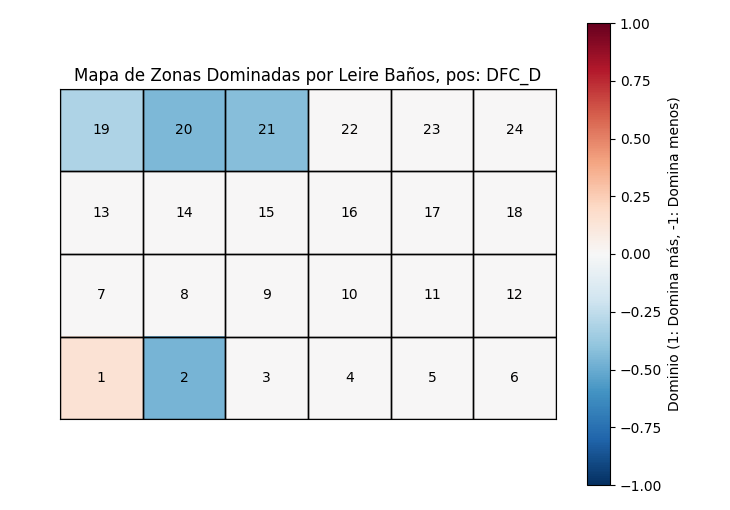
\includegraphics[width=0.7\textwidth]{plantilla-TFG-ETSIIT/doc/imagenes/futbolista_mapa_4.png}
    \caption{Mapa de influencia de Leire Baños}
    \label{fig:etiqueta-imagen}
\end{figure}

En este partido, se puede inferir que la defensa central por la derecha tuvo un desempeño deficiente, dado que no logró imponerse en las zonas centrales de la defensa, y solo mostró cierta efectividad en los laterales. Esta situación podría llevar al entrenador a concluir que la jugadora se vio obligada a salir de su posición habitual para brindar apoyo defensivo a las laterales, en especial al lateral izquierdo.

Estas interpretaciones son ejemplos de cómo un entrenador puede analizar distintas situaciones tácticas del juego, tales como coberturas, presión alta o ataques por las bandas. Asimismo, este análisis puede profundizarse para comprender el estilo de juego del rival. En definitiva, esta técnica ofrece una herramienta valiosa para que el cuerpo técnico prepare el partido de manera más efectiva.

\section{Algoritmos genético}
En esta sección se describe el proceso de ejecución de los algoritmos genéticos implementados para el análisis y predicción del rendimiento en los partidos. Se detallan los parámetros configurados, las etapas de evolución del algoritmo y la forma en que se manejan los datos para obtener resultados óptimos. 

Para poder explorar las distintas soluciones del problema, y para asegurarnos de que nos quedamos con la mejor, se va a ejecutar varias veces combinando los datos:

\begin{itemize}
    \item Población: El de tamaño de la población será de 40 u 80.
    \item El número de iteraciones que hace el algoritmo será de 20, 40 u 80.
    \item La tasa de mutación será de 1 ó 0.9.
\end{itemize}

Para llevar a cabo la ejecución, inicialmente se aplicará el algoritmo con una población de 40 individuos, 20 iteraciones y una tasa de mutación de 1. A continuación, se repetirá el proceso modificando únicamente la tasa de mutación a 0.9, y así sucesivamente hasta cubrir todas las combinaciones posibles. Dado que cada ejecución puede prolongarse durante varias horas, también se ha considerado relevante registrar el tiempo que tarda cada proceso.

Con el fin de garantizar la fiabilidad de los resultados y minimizar el impacto de la aleatoriedad, lo ideal sería ejecutar cada combinación 30 veces. Sin embargo, debido a limitaciones temporales, se ha optado por realizar cinco ejecuciones por combinación, lo que asegura un nivel mínimo de confianza. En el análisis de resultados no se mostrarán todas las tablas individuales, sino que se presentarán las medias obtenidas de las cinco ejecuciones junto con sus correspondientes desviaciones típicas.

\begin{table}[H]
\centering
\caption{Resultados del algoritmo genético para diferentes configuraciones}
\label{tab:resultados_algoritmo}
\begin{tabular}{|c|c|c|c|c|c|}
\hline
\textbf{Población} & \textbf{Generaciones} & \textbf{Cruzamiento} & \textbf{Mutación} & \textbf{Precisión (\%)} & \textbf{ejecución (min)} \\
\hline
40 & 20 & 1 & 1/48 & $85.02 \pm 0.67$  & 10\\
40 & 20 & 0.9 & 1/48 & $84.32 \pm 1.43$ & 10 \\
40 & 40 & 0.9 & 1/48 & $83.34 \pm 2.46$ & 19 \\
40 & 40 & 1 & 1/48 & $85.02 \pm 0.65$ & 19 \\

80 & 20 & 0.9 & 1/48 & $84.78 \pm 0.65$ & 19\\
40 & 20 & 1 & 1/48 & $85.98 \pm 1.07$ & 19 \\
40 & 80 & 1 & 1/48 & $85.5 \pm 1.2$& 36 \\
40 & 80 & 0.9 & 1/48 & $84.3 \pm 3.39$ & 36 \\

80 & 40 & 0.9 & 1/48 & $86.46 \pm 0.53$ & 36\\
40 & 40 & 1 & 1/48 & $85.98 \pm 0.65$ & 36 \\
80 & 80 & 1 & 1/48 & $86.94 \pm 0.53$ & 69 \\
80 & 80 & 0.9 & 1/48 & $86.46 \pm 0.53$ & 69 \\

\hline
\end{tabular}
\end{table}

Como se puede ver en la tabla, la mejor combinación es la de 80 individuos, 80 generaciones y tasa de cruzamiento de 1, con una precisión del 86,94\% y con una desviación típica de 0,53\%. Vamos a ver un gráfico de la evolución del algoritmo con esos parámetros.

\begin{figure}[H]
    \centering
    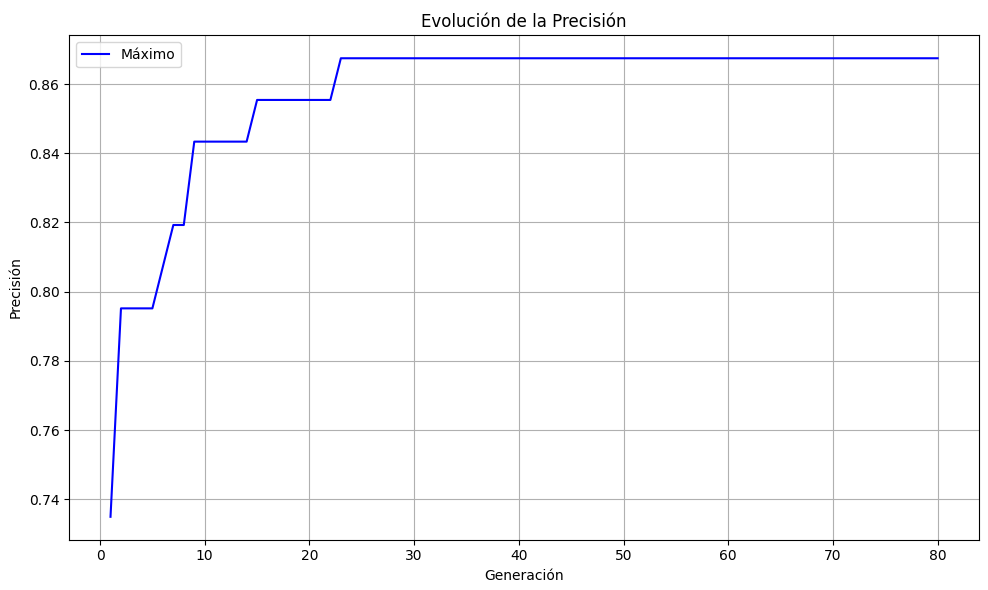
\includegraphics[width=1.0\textwidth]{plantilla-TFG-ETSIIT/doc/imagenes/Precision_gen.png}
    \caption{Gráfico algoritmo genético}
    \label{fig:etiqueta-imagen}
\end{figure}

Como se puede ver en el gráfico, el algoritmo evoluciona muy rápido, sin embargo, se estanca a partir de la generación 24. Los vectores que ha dado como resultado han sido los siguientes:

\begin{figure}[H]
    \centering
    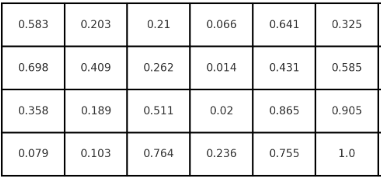
\includegraphics[width=0.7\textwidth]{plantilla-TFG-ETSIIT/doc/imagenes/Ataque_genetico.png}
    \caption{Vector de ataque genético}
    \label{fig:etiqueta-imagen}
\end{figure}

\begin{figure}[H]
    \centering
    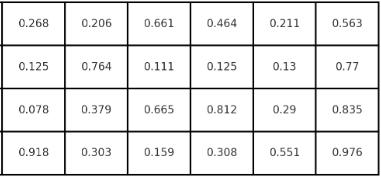
\includegraphics[width=0.7\textwidth]{plantilla-TFG-ETSIIT/doc/imagenes/Defensa_genetico.png}
    \caption{Vector de defensa genético}
    \label{fig:etiqueta-imagen}
\end{figure}

Como se puede observar, el vector de ataque incrementa a medida que el equipo avanza hacia el área rival, mientras que el vector de defensa se intensifica al retroceder hacia la propia. No obstante, existen ciertos valores atípicos, producto de la aleatoriedad inherente al fútbol, que no siguen este patrón. Aun así, es posible identificar una tendencia general. Además, se evidencia que la zona central del campo tiende a recibir menor atención estratégica en comparación con las áreas cercanas a las porterías.

\section{Algoritmo genético con $\delta$}
Para intentar que la predicción sea lo más precisa posible, vamos ahora a añadir al vector de pesos a $\delta$, que es la variable que representa en qué momento cortar para decidir si gana uno, otro o hay empate. Hasta ahora, esta variable había sido añadida a mano como 2, es decir, si:

\begin{itemize}
    \item $Score global > 2$, gana local
    \item $Score global < -2$, gana visitante
    \item empate en caso contrario
\end{itemize}

Ahora el algoritmo genético, aparte de definir los vectores de ataque y defensa para las ponderaciones de las zonas del campo, también va a decidir esta variable. La configuración del algoritmo es igual a la que se ha explicado antes, excepto para la tasa de mutación, que al añadir un nuevo valor al vector ha pasado a ser de 1/49. El objetivo es comparar técnicas y ver cuál es más rentable en cuanto a precisión y recursos.

Los distintos valores con los que se va a probar son los mismos que antes, se ha ejecutado un total de 5 veces y se ha calculado la media de cada combinación y su desviación típica.

\begin{table}[H]
\centering
\caption{Resultados del algoritmo genético con $\delta$ para diferentes configuraciones}
\label{tab:resultados_algoritmo}
\begin{tabular}{|c|c|c|c|c|c|}
\hline
\textbf{Población} & \textbf{Generaciones} & \textbf{Cruzamiento} & \textbf{Mutación} & \textbf{Precisión (\%)} & \textbf{ejecución (min)} \\
\hline
40 & 20 & 1 & 1/49 & $83.58 \pm 1.07$  & 13\\
40 & 20 & 0.9 & 1/49 & $83.6 \pm 1.03$ & 13 \\
40 & 40 & 0.9 & 1/49 & $83.58 \pm 0.65$ & 23 \\
40 & 40 & 1 & 1/49 & $85.02 \pm 1.37$ & 23 \\

80 & 20 & 0.9 & 1/49 & $85.5 \pm 1.47$ & 24\\
40 & 20 & 1 & 1/49 & $85.02 \pm 1.37$ & 24 \\
40 & 80 & 1 & 1/49 & $85.04 \pm 2.21$& 41 \\
40 & 80 & 0.9 & 1/49 & $84.78 \pm 1.37$ & 41 \\

80 & 40 & 0.9 & 1/49 & $86.22 \pm 0.65$ & 41\\
40 & 40 & 1 & 1/49 & $86.94 \pm 0.53$ & 41 \\
80 & 80 & 1 & 1/49 & $86.96 \pm 0.58$ & 86 \\
80 & 80 & 0.9 & 1/49 & $87.2 \pm 1.38$ & 86 \\

\hline
\end{tabular}
\end{table}

Como se puede apreciar, la mejor combinación es la de 80 individuos, 80 generaciones y tasa de cruzamiento 0.9 con una precisión del 87,2\% y una desviación típica de 1,38\%. El gráfico al ejecutarlo es el siguiente:

\begin{figure}[H]
    \centering
    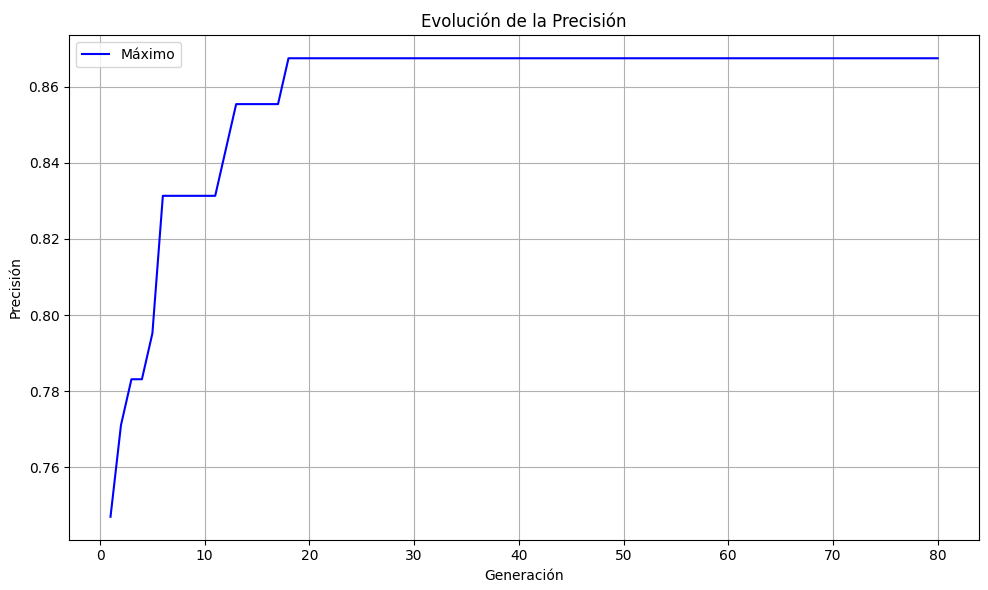
\includegraphics[width=0.7\textwidth]{plantilla-TFG-ETSIIT/doc/imagenes/Precision_delta.png}
    \caption{Grafico algoritmo genético}
    \label{fig:etiqueta-imagen}
\end{figure}

El gráfico es muy parecido al anterior, empieza evolucionando rápido, sin embargo, a partir de la generación 18 se estanca y no consigue avanzar más. Los vectores resultado son:

\begin{figure}[H]
    \centering
    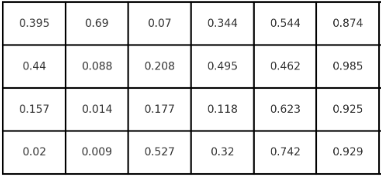
\includegraphics[width=0.7\textwidth]{plantilla-TFG-ETSIIT/doc/imagenes/Ataque_gen_delta.png}
    \caption{Vector de ataque genético con $\delta$}
    \label{fig:etiqueta-imagen}
\end{figure}

\begin{figure}[H]
    \centering
    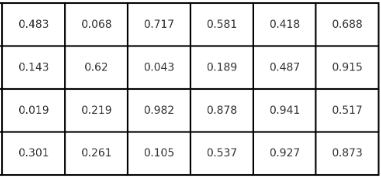
\includegraphics[width=0.7\textwidth]{plantilla-TFG-ETSIIT/doc/imagenes/Defensa_gen_delta.png}
    \caption{Vector de defensa genético con $\delta$}
    \label{fig:etiqueta-imagen}
\end{figure}

Los resultados de los vectores muestran un comportamiento similar al anterior: se otorga mayor relevancia a las áreas cercanas a las porterías que al centro del campo, aunque persisten ciertos valores aleatorios derivados de la impredecibilidad inherente al fútbol. Para determinar al ganador, se ha establecido un valor de corte, que se corresponde con $\delta$ de 1.75, ligeramente inferior al fijado manualmente en análisis previos, pero dentro de un rango comparable.

\section{Simetría de zonas}
Resulta llamativo que en la sección 6.5, dedicada a la ejecución del algoritmo genético, los resultados obtenidos presenten una marcada asimetría. Esta podría deberse a diversos factores, como la aleatoriedad inherente al fútbol, la tendencia de algunos equipos a atacar preferentemente por una banda concreta o, simplemente, a una coincidencia puntual.

En cualquier caso, se ha considerado oportuno analizar qué ocurriría si se partiera de un mapa con zonas simétricas. Para ello, se calculó la media de las zonas simétricas de los vectores generados por el algoritmo genético, tanto en ataque como en defensa. Posteriormente, se simularon todos los partidos de la base de datos utilizando estos pesos promedio, y a continuación se presentan los resultados obtenidos.

\begin{figure}[H]
    \centering
    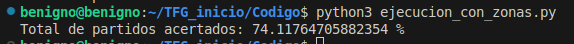
\includegraphics[width=0.7\textwidth]{plantilla-TFG-ETSIIT/doc/imagenes/zonas_simetricas.png}
    \caption{Ejecución con vectores simétricos}
    \label{fig:etiqueta-imagen}
\end{figure}

El resultado obtenido, del 74,11\%, mejora el rendimiento del sistema basado en la selección manual de pesos, aunque sigue siendo inferior al alcanzado por el algoritmo genético.

Puede considerarse un resultado aceptable en términos de predicción de partidos, si bien presenta una menor precisión en comparación con otros métodos más optimizados. Probablemente, la asimetría observada en los resultados esté relacionada con las dinámicas del fútbol moderno, en el que los equipos adoptan estrategias cada vez más complejas y tienden a concentrar su juego en determinadas zonas del campo, en lugar de mantener una distribución homogénea.

Por tanto, se valora la posibilidad de introducir ajustes adicionales en el modelo que permitan capturar mejor estas asimetrías, así como explorar variantes del algoritmo que integren este tipo de patrones estratégicos.

\section{Conclusión}
En términos generales, no se observa una diferencia significativa entre ambos algoritmos genéticos, lo que sugiere que el umbral utilizado para determinar el ganador a partir del puntaje global no resulta determinante. Esto probablemente se deba a que cada partido presenta valores variables, mayores o menores, en función de su desarrollo, y las puntuaciones de los equipos se adaptan a dichas circunstancias, evitando que exista una tendencia fija en el puntaje global.

Por otro lado, el porcentaje de acierto alcanzado, de $87.2 \pm 1.38$, es considerablemente alto para el contexto del fútbol, lo que permite afirmar con satisfacción que se ha logrado cumplir el objetivo principal planteado en este Trabajo de Fin de Grado.

        \chapter{Conclusiones y trabajos futuros}


	
	\newpage
	\bibliography{bibliografia}
	\bibliographystyle{plain}
	
\end{document}

